\newpage
\section{Introduzione analisi in più variabili}
Fin'ora abbiamo visto: insiemi $\subset \mathbb{R}$, funzioni da $\mathbb{R}\to \mathbb{R}$ con i imiti di funzioni ed il calcolo differenziale, teoria dell'integrazione per funzioni di una variabile, successioni e serie numeriche. L'ultima parte del corso l'obbiettivo è lavorare con più variabili in particolare con $\mathbb{R}^n$, vorremmo definire l'insieme nel piano (nello spazio), derivare delle curve e studiare funzioni in più variabili $f: \mathbb{R}^n \to \mathbb{R}$ quindi definire un limine la continuità, le derivare e studiare la funzione individuando massimi e minimi.
\subsection{Struttura euclidea di $\mathbb{R}^n$}
\begin{definition}
Possiamo definire $\mathbb{R}^n$ come uno spazio vettoriale dove possiamo fare somma, prodotto per un numero, combinazioni lineare indipendenza lineare, la base ed i sottospazi. Se $x \in \mathbb{R}^n \rightarrow x = (x_1, x_2, ..., x_n)$.
\end{definition}
\hspace{-15pt}Per esempio $x = (x_1, x_2)\in \mathbb{R}^2$, mentre $x = (x_1, x_2, x_3) \in \mathbb{R}^3$. Alle livello di notazioni si può scrivere $\mathbb{R}^2 = (x,y) \in \mathbb{R}^2$. \\
$\mathbb{R}^2$ sarà un piano mentre $\mathbb{R}^3$ sarà uno spazio dove possiamo definire.
\begin{itemize}
    \item Somma di 2 vettori: $x = (x_1, ..., x_n)$, $y = (y_1, ..., y_n)$, e $x + y = (x_1 + y_1, ..., x_n + y_n)$.
    \item Prodotto per un numero $\lambda \in \mathbb{R}$: $\lambda \cdot x = (\lambda \cdot x_1, \lambda \cdot x_2, ..., \lambda\cdot x_n)$.
\end{itemize}

\subsection{Operazioni sullo spazio}
Definiamo una la struttura di questo spazio, e lo facciamo definendo delle operazioni.
\begin{definition}[Prodotto scalare]
Il \textbf{prodotto scalare} è un operazione che ha come input 2 vettori, dato $x,y \in \mathbb{R}^n$ definiti come $x= (x_1, ..., x_n), y = (y_1, ..., y_n)$ il prodotto scalare è:
\vspace{-10pt}
\[<x, y> = x \cdot y = (x, y) = x_1y_2 + x_2y_2 + x_3y_3 + ... + x_ny_n = \sum\limits_{i=1}^n x_iy_i\]
\end{definition}
\begin{definition}[Norma]
La \textbf{norma} è un operazioni che ah come input un solo vettore e come risultato un numero maggiore o uguale a 0. Dato $x \in \mathbb{R}^n$, $x = (x_1, x_2, ..., x_n)$ la norma è:
\[||x|| = |x| = \sqrt{<x,x>} = \sqrt{x_1^2 + x_2^2 + ... + x_n^2}\]
La norma di x è la lunghezza del vettore x.
\end{definition}
\begin{definition}[Distanza]
La \textbf{distanza} è un'operazione che ha come input due vettori e come risultato un numero maggiore o uguale a 0. Dato un $x,y \in \mathbb{R}^n$ definiamo la distanza come:
\[dist(x,y) = d(x,y) = ||x - y|| = \sqrt{(x_1 - y_1)^2 + (x_2 - y_2)^2 + ... + (x_n - y_n)^2}\]
\end{definition}

\hspace{-15pt}Notare che con queste operazioni abbiamo definito in $\mathbb{R}^n$:\\
(misurare gli angoli)$<,> \xrightarrow[]{\text{induce}}$ (lunghezza di un vettore) $|| . || \xrightarrow[]{\text{induce}}$ (distanza tra due elementi) $d$
Il prodotto scalare serve a misurare gli angoli perché geometricamente $<x,y> = ||x|| \cdot ||y|| \cdot \cos{\Theta}$ dove $\Theta$ è l'angolo compreso fra i vettori $x,y$.
\begin{note}
Una piccola digressione per dire che possiamo dire sia punti $(x_1, x_2)$ oppure il punto $x$ è uguale dove in $\mathbb{R}^2$ se scrivo $(x_1, x_2)$ questo rappresenta sia il punto che il vettore applicato nell'origine come punto della freccia in $(x_1, x_2)$.
\end{note}
\begin{wrapfigure}[4]{r}{6cm}
    \vspace{-20pt}
    \centering
    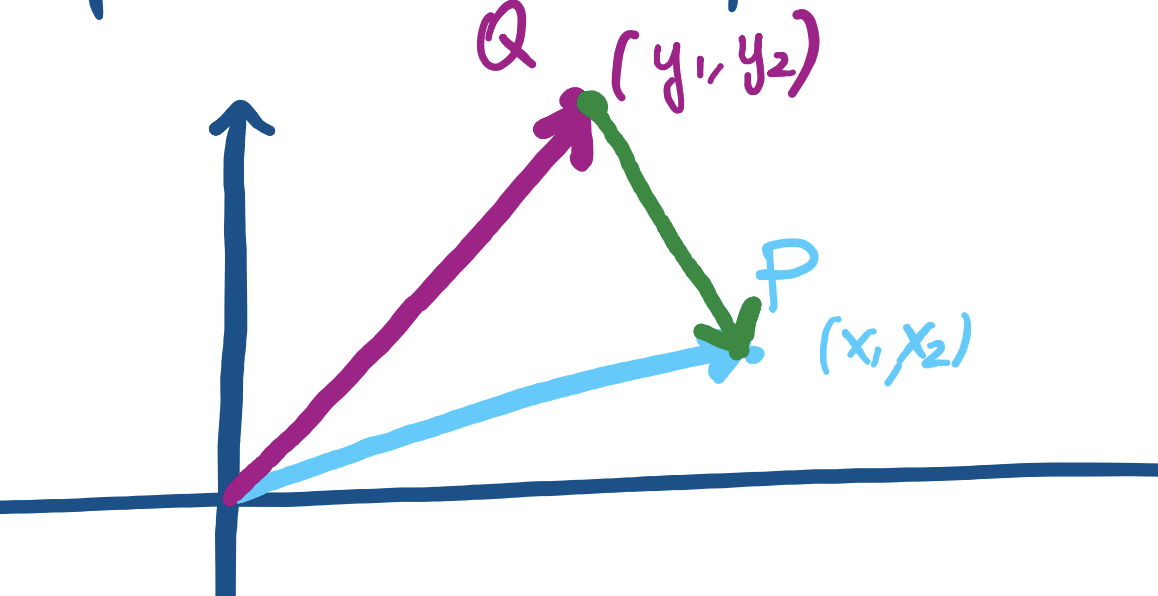
\includegraphics[width=5cm]{images/ess-vettore.png}
\end{wrapfigure}
In questa rappresentazione la differenza tra i due vettori P, Q dove $P \leftrightarrow x = (x_1, x_2)$ e $Q \leftrightarrow y = (y_1, y_2)$, è $x-y = (x_1 - y_1, x_2 - y_2) = \vec{P} - \vec{Q}$ (penso il vettore differenza come applicato un Q con punta della freccia in P). Quindi $d(x,y) = d(P,Q) = ||x-y||$.

\subsection{Insiemi nello spazio $\mathbb{R}^n$}
Data la nozione di distanza possiamo definire gli insiemi in uno spazio $\mathbb{R}^n$.
\begin{definition}[Palla]
Dato $x \in \mathbb{R}^n$ e dato $r > 0, r \in \mathbb{R}$ si dice \textbf{palla} di centro x e raggio r:
\[B(x,r) = B_r(x) = \{y \in \mathbb{R}^n \::\: d(x,y) < r\}\]
La palla di centro x e raggio r può essere chiamato anche intorno sferico di x di raggio r.
\end{definition}
\hspace{-15pt}Per esempio in caso di $\mathbb{R}^2$, $B(x,r) = B_r(x) = \{y \in \mathbb{R}^2 \::\: d(x,y) < r\}$, sarà una circonferenza escluso il bordo. Nel caso di $\mathbb{R}^3$ invece sarà una sfera piena privata del bordo.\\
Se torniamo al caso $\mathbb{R}$ la $B_r(x) = \{\in \mathbb{R} \::\: d(x,y) < r\}$ dove $d(x,y) = |x-y|$, quindi come il caso $\mathbb{R}^n$ solo che nel caso di $\mathbb{R}$ abbiamo un valore assoluto mentre nel caso $\mathbb{R}^n$ abbiamo una norma.

\begin{figure}[h!]
\centering
\begin{subfigure}{.45\textwidth}
    \centering
    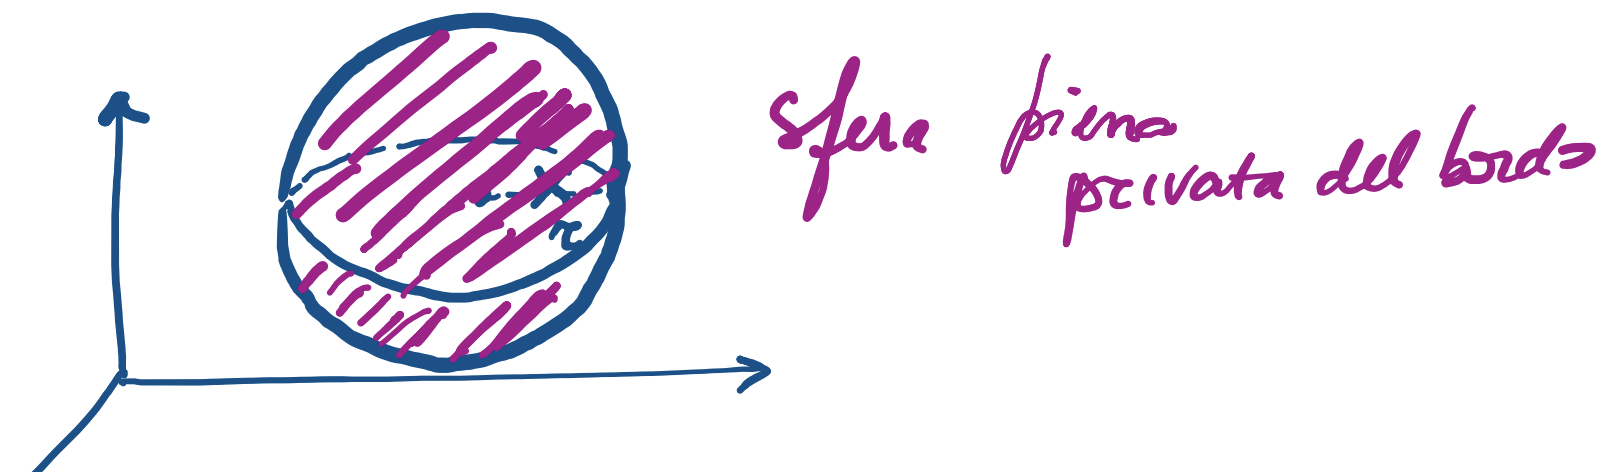
\includegraphics[width=6cm]{images/sfera-piena-priva-bordo.png}
    \caption{Sfera piena priva di bordo}
\end{subfigure}
\begin{subfigure}{.45\textwidth}
    \centering
    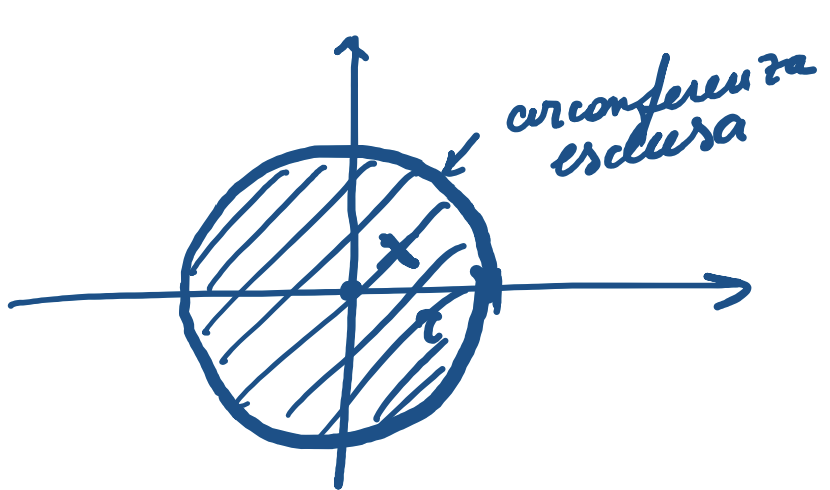
\includegraphics[width=4cm]{images/circonferenza-esclusa.png}
    \caption{Circonferenza esclusa}
\end{subfigure}
\end{figure}

\begin{definition}[Sfera]
Dato $x \in \mathbb{R}^n$. e dato $r > 0, r \in \mathbb{R}$ si dice \textbf{sfera} di centro x e raggio r l'insieme:
\[S(x,r) = S_r(x) = \{y \in \mathbb{R}^n \::\: d(x,y) = r\}\]
\end{definition}
\hspace{-15pt}Nel caso vedessimo la sfera in $\mathbb{R}$ avremmo $S_r(x) = \{x-r\} \cup \{x + r\}$.

\begin{figure}[h!]
    \centering
    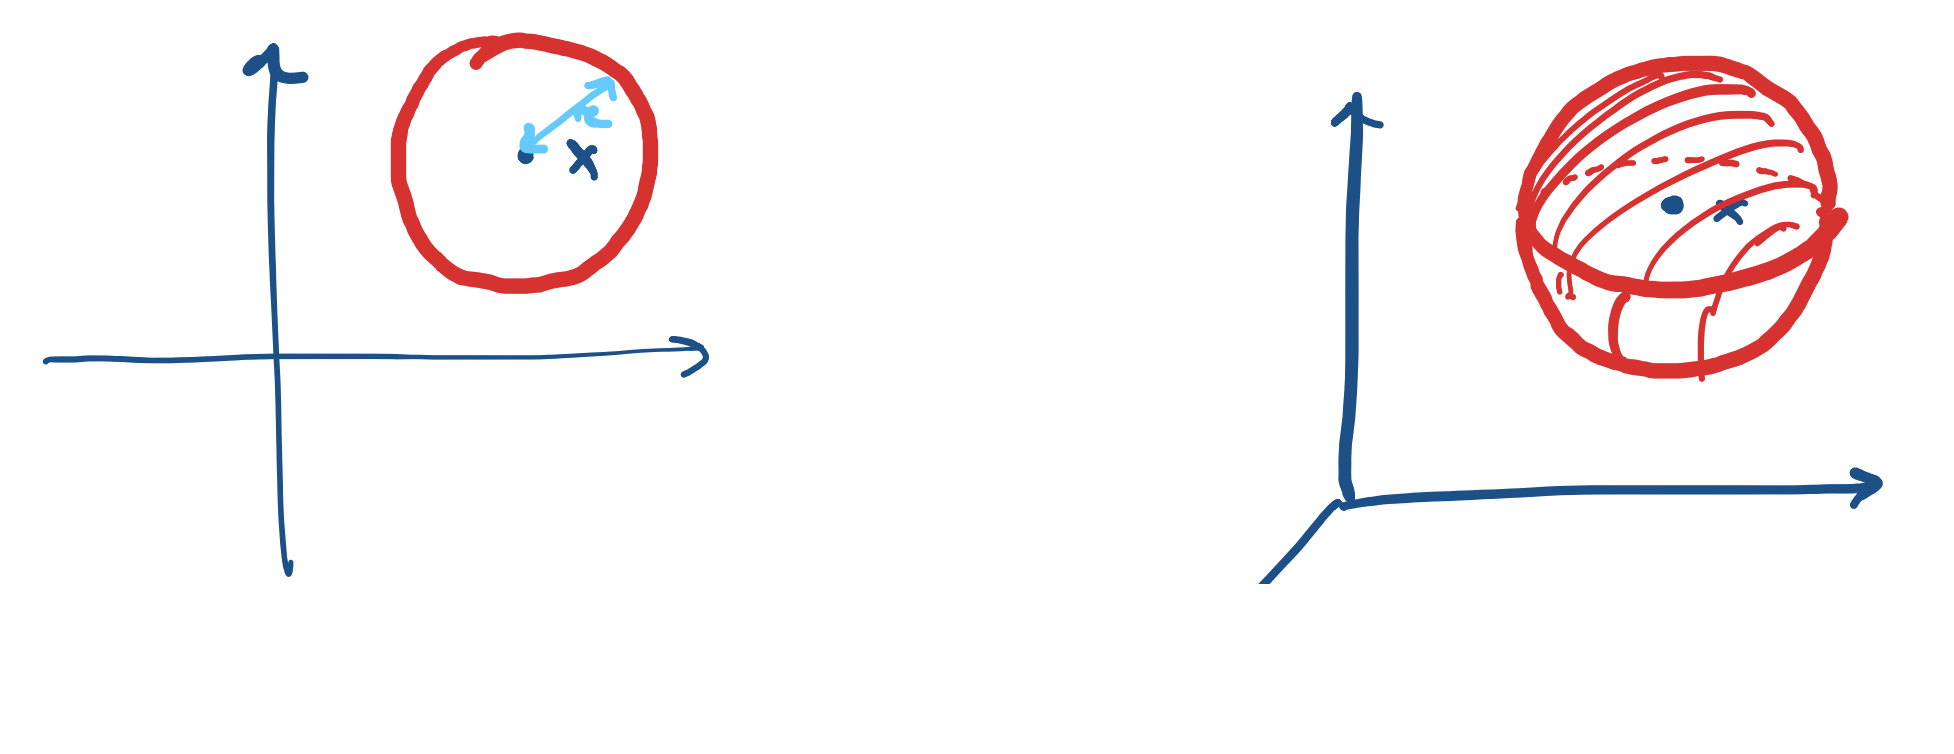
\includegraphics[width=9cm]{images/ess-sfera.png}
    \vspace{-20pt}
    \caption{Esempi sfera}
\end{figure}

\vspace{-10pt}
\subsection{Proprietà di $\mathbb{R}^n$}
Ricordiamo come notazione che se $E$ è un insieme $E \subseteq \mathbb{R}^n$ allora indichiamo ocn $E^c = \mathbb{R}^n \setminus E =$ complementare di E rispetto a tutto $\mathbb{R}^n$.
\begin{definition}[Punto interno, esterno, di frontiera]
Sia $E \subseteq \mathbb{R}^n$ un punto $x_0 \in \mathbb{R}^n$ si dice:
\begin{itemize}
    \item \textbf{Punto interno ad E} se esiste una palla di centro $x_0$ e raggio $r > 0$ contenuta in E, cioè se esiste $r > 0$ tale che $B_r(x_0) \subset E$, si dice che $x_0$ è un punto interno ad E.
    \item \textbf{Punto esterno ad E} se esiste una palla di centro $x_0$ e raggio $r$ tutta contenuta in $E^x$ cioè se $\exists r > 0$ tale che $B_r(x_0) \subset E^c = R^n \setminus E$.
    \item \textbf{Punto di frontiera per E} se non è ne interno ne esterno. $\forall r > 0$ $V_r(x_0) \cap E \neq \O$ e $B_r(x_0) \cap E^c \neq \O$.
\end{itemize}
\end{definition}

\begin{observation}
Alcune osservazioni su queste proprietà:
\begin{itemize}
    \item Se $x_0$ è un punto interno ad E $\Longrightarrow x_0 \in E$.
    \item Se $x_0$ è punto esterno ad E $\Longrightarrow x_0 \notin E$.
    \item Se $x_0$ è punto di frontiera $\Longrightarrow x_0 \in E$ oppure $x_0 \notin E$.
\end{itemize}
\end{observation}
\hspace{-15pt}A livello di notazione si indica $\mathring{E}$ l'insieme dei punti interni, e con $\delta E$. l'insieme dei punti di frontiera di E.

\begin{example}
Dato E = $\{x \in \mathbb{R}^2 \::\: x = (x_1, x_2) \::\: x_2> 0 \}$. Ci chiediamo quali siano $\mathring{E}$, $\delta E$ e l'insieme dei punti esterni.
\end{example}

\begin{figure}[h!]
    \centering
    \vspace{-10pt}
    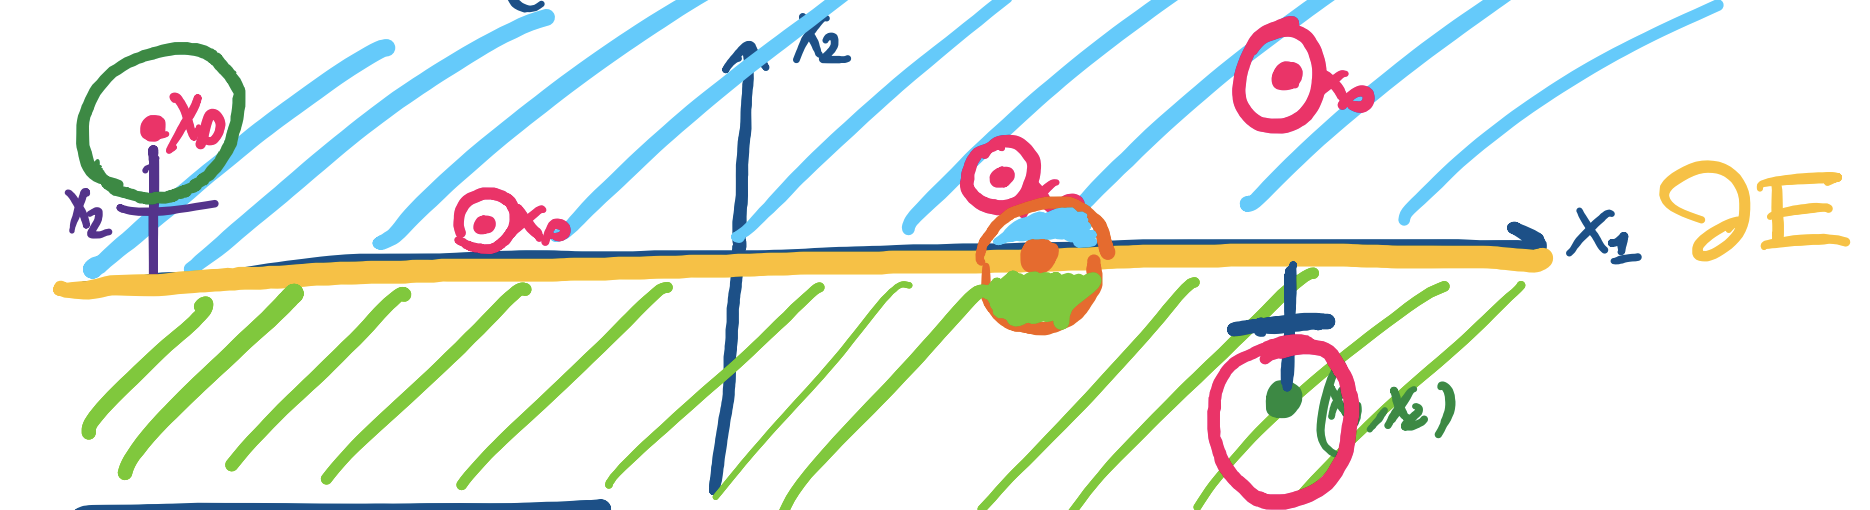
\includegraphics[width=8cm]{images/ess-punti-interni.png}
\end{figure}

\vspace{-10pt}
\begin{itemize}
    \item L'insieme dei punti interni $\mathring{E} = E$. Per dimostrare prendo $(x_1, x_2) \in E$ appartenendo ad E ho che $x_2 > 0$ quindi scelgo $r < \frac{x_2}{2} \Longrightarrow B_r(x_0) \subset E \rightarrow E x_0 \in \mathring{E}$ quindi ho dimostrato che $E \subset \mathbb{E}$ e quindi $E = \mathring{E}$. In questo caso tutti i punti di E sono punti interni ad E (il viceversa è sempre vero).
    \item $\delta E = \{(x_1, x_2) \in \mathbb{R}^2 \::\: x_2 = 0\}$ questo è vero perché qualsiasi punto i prenda fra i punti di frontiera andrò ad intersecare sia E che il suo complementare. 
    \item A questo punto l'insieme dei punti esterni $= A = \{(x_1, x_2) \in \mathbb{R}^2 \::\: x_2 < 0\}$. Per verificare di chiediamo se i punti esterni $\in E^c$, voglio dimostrare che se $A \subset$ punti esterni allora $(x_1, x_2) \in A$, $x_2 < 0 \rightarrow$ scelgo $r < \frac{|x_2|}{2}$, quindi $B_r (x_1, x_2)\subset E^c$ ed allora ho dimostrato che $(x_1, x_2)$ è punto esterno. 
\end{itemize}

\begin{example}
Prendo $E = \{(x_1, x_2) \in \mathbb{R}^2 \::\: 1 < x_1^2 + x_2^2 \leq 4\}$. L'esercizio consiste nel calcolare $\mathring{E}$, $\delta E$ e l'insieme dei punti esterni di E.
\end{example}

\subsection{Punto di accumulazione}
\begin{definition}[Punto di accumulazione]
\end{definition}
\begin{wrapfigure}[4]{r}{6cm}
    \vspace{-45pt}
    \centering
    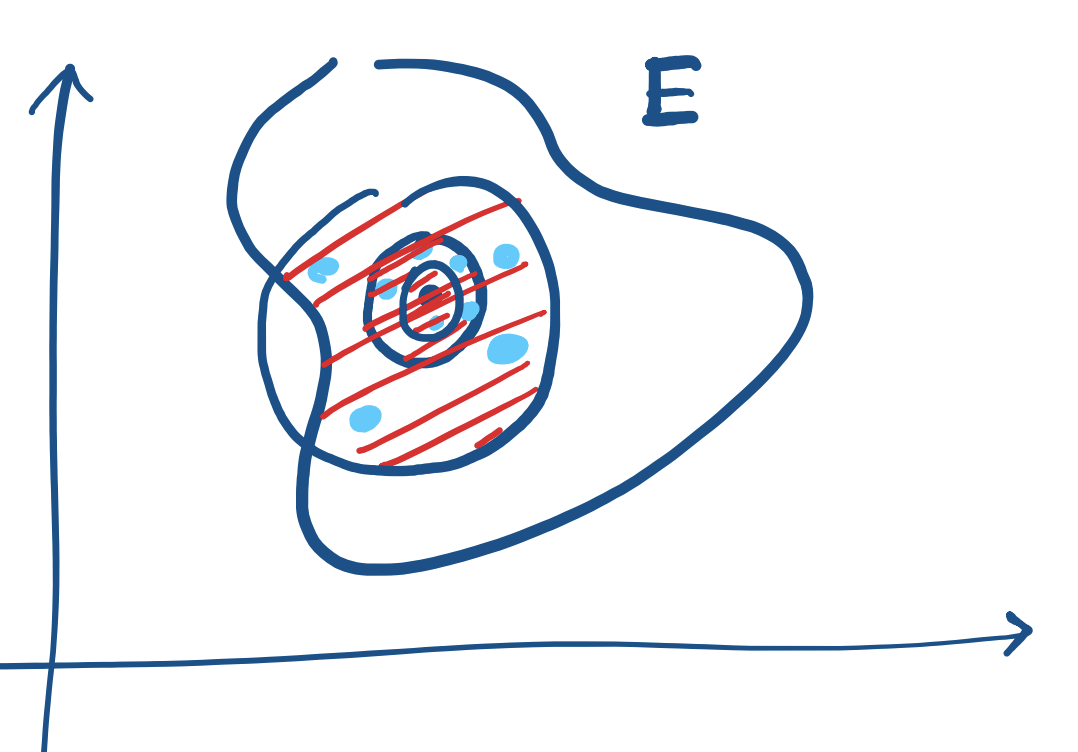
\includegraphics[width=4cm]{images/punti-accumulazione.png}
\end{wrapfigure}
\hspace{-15pt}Dato $E \subset \mathbb{R}^n$ un punto $x \in \mathbb{R}^n$ si dice \textbf{punto di accumulazione} per E se ogni palla di centro x esiste un punto di E diverso da x. Questo è vero se e solo se $\forall r > 0, B_r(x) \cap E \setminus \{x_0\} \neq \O$.

\begin{observation}
Osserviamo che se un punto è interno $\Longrightarrow$ è punto di accumulazione.
\end{observation}

\begin{definition}[Punto isolato]
Se un punto di E non di accumulazione per E allora si dice \textbf{punto isolato}.
\end{definition}

\begin{definition}[Insieme aperto e chiuso]
Possiamo definire dato un insieme E $\subseteq \mathbb{R}^n$ che 
\begin{itemize}
    \item Questo insieme si dice \textbf{aperto} se ogni $x \in E$ è punto interno ad E cioè $E= \mathring{E}$.
    \item Questo insieme si dice \textbf{chiuso} se $E^c$ è aperto.
\end{itemize}
\end{definition}

\begin{example}
Alcuni esempi di insiemi aperti e chiusi.
\begin{itemize}
    \item $E= \{(x_1, x_2) \in \mathbb{R}^2 \::\: x_1 > 0\}$ è aperto.
    \item $E = \{(x_1, x_2) \in \mathbb{R}^2 \::\: x_1 \geq 0\}$ è chiuso.
\end{itemize}
\end{example}

\begin{theorem}
Se E contiene tutto $\delta E \Longleftrightarrow E$ è chiuso. Quindi diciamo che $\delta E \subset E \Longrightarrow E$ chiuso.
\end{theorem}

\begin{example}
Qualche altro esempio.
\begin{itemize}
    \item $E= \{(x_1, x_2) \in \mathbb{R}^2 \::\: x_1^2 + x_2^2 < 1\}$ è aperto. La frontiera è $\gamma E = \{(x_1, x_2) \::\: x_1^2 + x_2^2 = 1\}$.
    \item $E= \{(x_1, x_2) \in \mathbb{R}^2 \::\: 2x_1 + 3x_2 -1 = 0\}$, $2x_1 + 3x_2 -1 = 0$ è una retta quindi $E = \gamma E$ ed è chiuso.
\end{itemize}
\end{example}

\subsection{Proprietà insiemi aperti e chiusi}
Alcune proprietà degli insiemi aperti di $\mathbb{R}^n$:
\begin{itemize}
    \item Sia $\O$ che $\mathbb{R}^n$ sono considerati insiemi aperti.
    \item L'unione (anche numerabile) è aperta. Quindi se prendo $E_1, ..., E_n, ...$ aperti $\cup_{n \in \mathbb{N}}E_n = E$ è aperta.
    \item L'intersezione (finita) di insiemi aperti è un insieme aperto.
\end{itemize}
Alcune proprietà degli insiemi chiusi di $\mathbb{R}^n$:
\begin{itemize}
    \item Sia $\O$ che $\mathbb{R}^n$ sono considerati anche chiusi.
    \item L'unione finita di insiemi chiusi è un insieme chiuso.
    \item L'intersezione (anche numerabile) di un insiemi chiusi è chiusa.
\end{itemize}

\subsection{Insieme limitato}
\begin{definition}[Insieme limitato]
Un insieme $E \subseteq \mathbb{R}^n$ si dice \textbf{limitato} se esiste un palla di centro l'origine che contiene tutto E. Ovvero se $\exists r > 0$ tale che $E \subset B_r(0)$.
\end{definition}

\begin{example}
Ad esempio se prendiamo un quadrato $\subseteq \mathbb{R}^2$ è limitato. Mentre invece una retta $\subseteq \mathbb{R}^2$ non è limitata.
\end{example}

\begin{definition}[Intorno]
Un intorno di raggio r sferico di $\infty$ (o la palla di centro $\infty$ e raggio r) è il complementare della palla chiusa di $\mathbb{R}^n$ con centro l'origine e raggio r.
\end{definition}

\begin{example}
Prendiamo per esempio $\mathbb{R}^2$, si ha $B_r(x) = \{y \in \mathbb{R}^n \::\: d(x,y)<r\}$.\\
Se prendo invece centro $x = \infty$, si ha $B_r(\infty) = \mathbb{R}^n \setminus \overline{B_r(0)}$. $\forall \overline{B_r(0)}$ trovo un intorno sferico di $\infty$ definito come $\mathbb{R}^n \setminus B_r(0)$.
\end{example}

\begin{observation}
Avendo introdotto $\mathbb{R}^n$ e ricordando la definizione di punto di accumulazione cioè $E \subseteq \mathbb{R}^n$, x si dice di accumulazione per E se in ogni palla di centro x esiste un punto E diverso da x. Un insieme non è limitato se e solo se $\infty$ è punto di accumulazione.
\end{observation}
\begin{wrapfigure}[4]{r}{6cm}
    \vspace{-25pt}
    \centering
    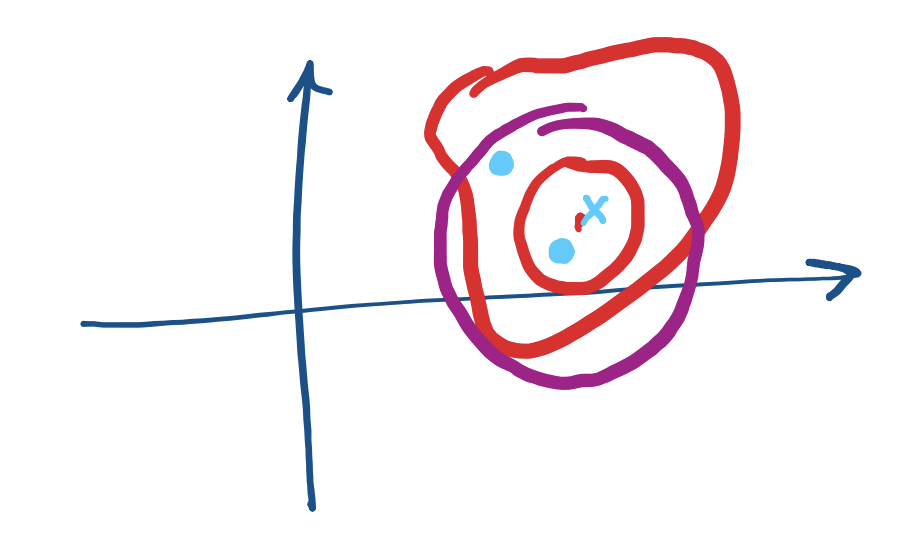
\includegraphics[width=5.5cm]{images/oss-punto-accumulo.png}
\end{wrapfigure}
Questo perché $\infty$ è punto di accumulazione $\Longleftrightarrow$ comunque grande io prenda la palla di centro 0 quando vado a prendere il suo complementare continuo a trovare punti che si intersecano con E. Vuol dire che E non può essere chiuso in una palla di centro 0.

\subsection{Oggetti su un piano $\mathbb{R}^2$}
\begin{wrapfigure}[4]{l}{5cm}
    \vspace{-20pt}
    \centering
    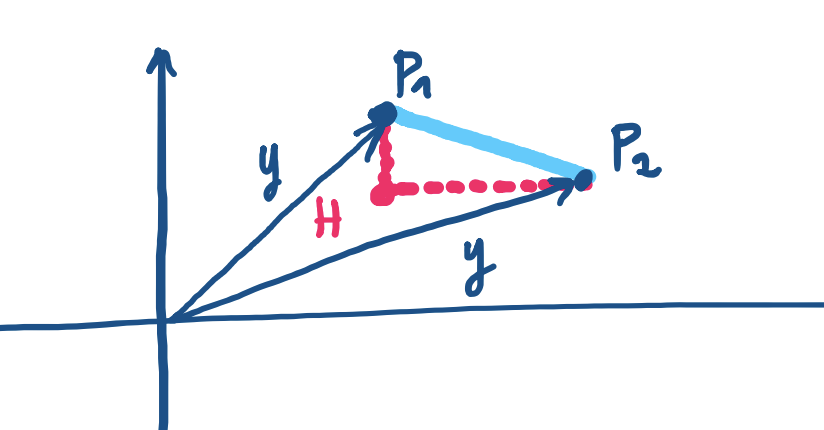
\includegraphics[width=4cm]{images/piano_R2.png}
\end{wrapfigure}
Ricordiamo ora che se prendiamo un piano $\mathbb{R}^2$, e due vettori $P_1 = x = (x_1, x_2)$, $P_2 = y = (y_1, y_2)$, la distanza $d(P_1, P_2) = \sqrt{(x_1 - x_2)^2 + (y_1-y_2)^2}$, e questo viene dal teorema di Pitagora dove $(P_1P_2)^2 = (P_1H)^2 + (P_2H)$.

\subsubsection{Retta per 2 punti}
\begin{wrapfigure}[4]{r}{5cm}
    \vspace{-20pt}
    \centering
    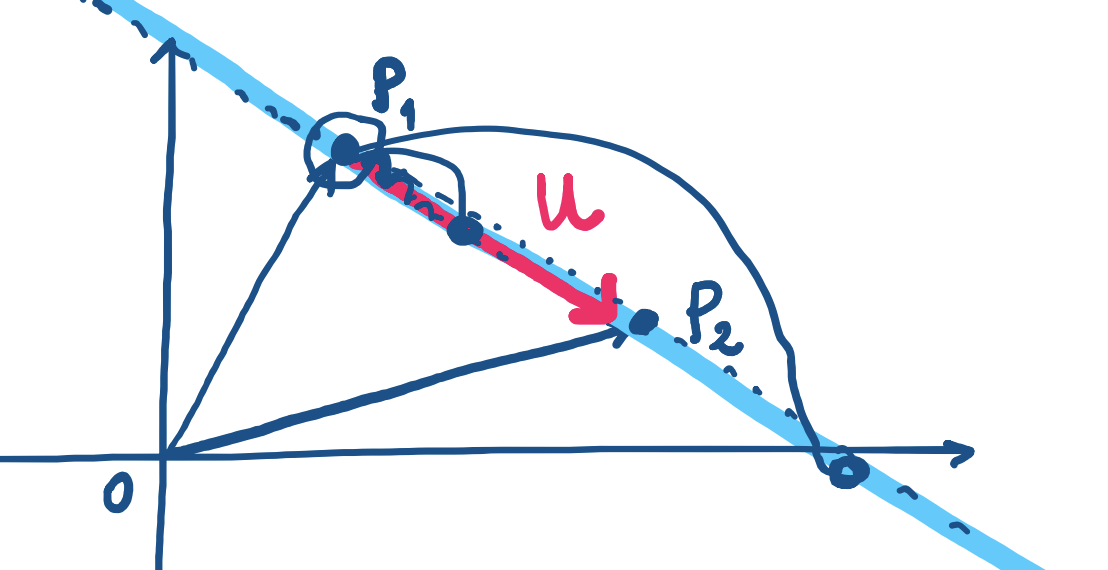
\includegraphics[width=4.5cm]{images/retta-2-punti.png}
\end{wrapfigure}
Prendiamo un piano con $P_1 = (x_1, y_1) = v$, $P_2 = (x_2, y_2) = w$. Noi vogliamo scrivere l'equazione di una retta che passa per due punti del piano. Per descrivere questa retta chiamiamo $u = w - v$, la retta è l'insieme dei punti che ottengo partendo da $P_1$ e spostandomi in direzioni di u. Analiticamente:
\[Retta = \{P_{t\in \mathbb{R}} = v + tu\} \text{ dove t è un paramento} = \Bigg\{\begin{pmatrix}x\\y\end{pmatrix} = \begin{pmatrix}x_1\\y_y\end{pmatrix} + t\begin{pmatrix}x_2 - x_1\\y_2 - y_y\end{pmatrix}\Bigg\}\]
Questa forma in cui ho descritto la retta si chiama \textbf{forma parametrica} della retta passante per $P_1$ e $P_2$, perché usiamo un parametrica p. Da qui possiamo scrivere la forma cartesiana:
\[\begin{cases}x = x_1 + t(x2 - x_1)\\ y = y_1 + t(y_2 - y_1)\end{cases} = \begin{cases}t = \frac{x - x_1}{x_2 - x_1}\\t = \frac{y - y_1}{y_2 - y_1}\end{cases} = \frac{x-x_1}{x_2 - x_1} = \frac{y - y_1}{y_2 - y_1}\]
Questa ultima forma senza t si chiama appunto \textbf{forma cartesiana} della retta passante per $P_1$ e $P_2$.
\[x-x_1 = \frac{(y - y_1)(x_2 - x_1)}{y_2 - y_1} = y\frac{(x_2 - x_1)}{y_2 - y_1} - \frac{y_1(x_2 - x_1)}{y_2 - y_1}\]
\[x - y\frac{x_2 - x_1}{y_2 - y_1} + \frac{y_1(x_2 - x_1)}{y_2 - y_1} - x_1 = 0 \rightarrow ax + by + c = 0\:\:  \text{ almeno uno tra a e b deve} \neq 0\]
\begin{observation}
Nella forma $ax + by + c = 0$ due equazioni rappresentato la setta retta $\Longleftrightarrow$ sono l'una multipla dell'altra.
\end{observation}

\subsubsection{Retta perpendicolare a v passante per l'origine}
Quindi siamo sempre nel piano ed abbiamo un vettore $v = (a,b)$, (in questo caso al posto di $x_1, x_2$ uso a,b). Individuo il vettore $w \perp v$ passante per l'origine e descrivo $r: \{P = t\cdot w, t \in \mathbb{R}\}$. \\
\begin{wrapfigure}[8]{r}{6cm}
    \vspace{-20pt}
    \centering
    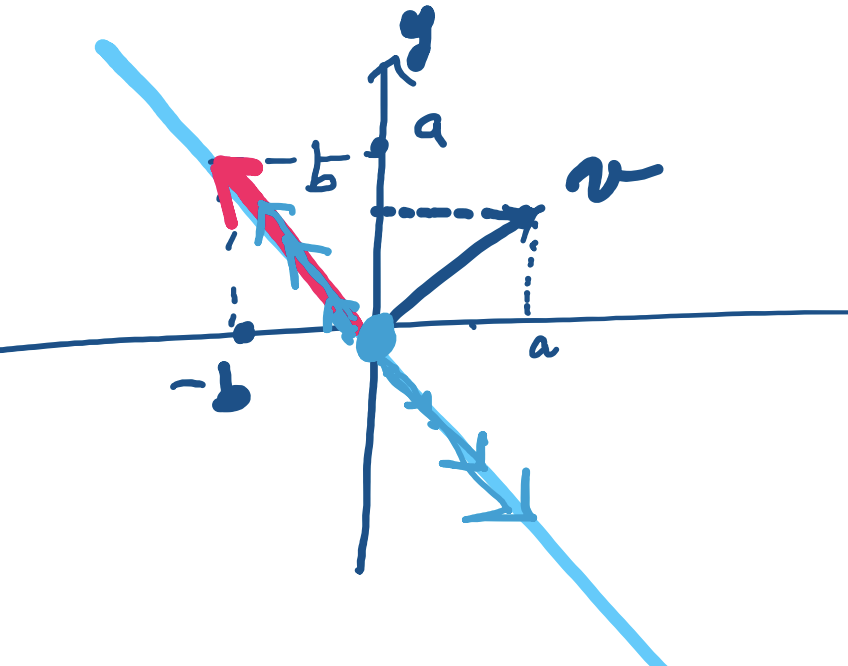
\includegraphics[width=4.5cm]{images/retta-perpendicolare-in-R3.png}
\end{wrapfigure}
Per trovare w partiamo dal fatto che abbiamo visto che $v \perp w \Longleftrightarrow <v,w> = 0$ se do' a w due componenti $w = (w_1, w_2)$ sto cercando $w_1$ e $w_2$ tali che $w \perp v$, a questo punto posso imporre la condizione $<(a,b), (w_1, w_2)> = 0$ che è $a \cdot w_1 + b \cdot w_2 = 0$, mi accorgo che posso scegliere $w_1 = -b$ e $w_2 = a$ ed in questo modo ho $<v,w> = a \cdot (-b) + b \cdot a = 0$ quindi ricapitolando w è determinato da v ed è $w = (-b,a)$ tale che $w \perp v$ (anche $-w = (a, -b) \perp v$) quindi adesso:
\[r = \{P = t \cdot w\ = \{\begin{pmatrix}x\\t\end{pmatrix}\in \mathbb{R}^2 \::\: \begin{pmatrix}x\\y\end{pmatrix}=t \cdot \begin{pmatrix}-b\\a\end{pmatrix}\}\]
Questa è detta forma parametrica perché abbiamo appunto un parametro t. Da questa forma possiamo ricavare la forma cartesiana.
\[\begin{cases}x = -tb \\ y = ta\end{cases} = \begin{cases}t = \frac{y}{a}\\ y= -\frac{y}{a}\cdot b\end{cases} = ax + by = 0\]
\begin{observation}
Vediamo una serie di osservazioni.
\begin{enumerate}
    \item $ab + by = 0$ è una forma cartesiana della retta passante per l'origine $\Longleftrightarrow c = 0$, $e \perp a$, $v = (a,b)$.
    \item Data una retta $ax + by + c = 0 \rightarrow v = (a,b)$ è $\perp r$.
\end{enumerate}
\end{observation}

\subsubsection{Retta tangente ad un grafico}
Siamo sempre in $\mathbb{R}^2$ e supponiamo di avere una funzione $f: \mathbb{R}\to \mathbb{R}$ continua, derivabile e con derivate continue in tutto $\mathbb{R}$.\\
\begin{wrapfigure}[7]{l}{6cm}
    \vspace{-10pt}
    \centering
    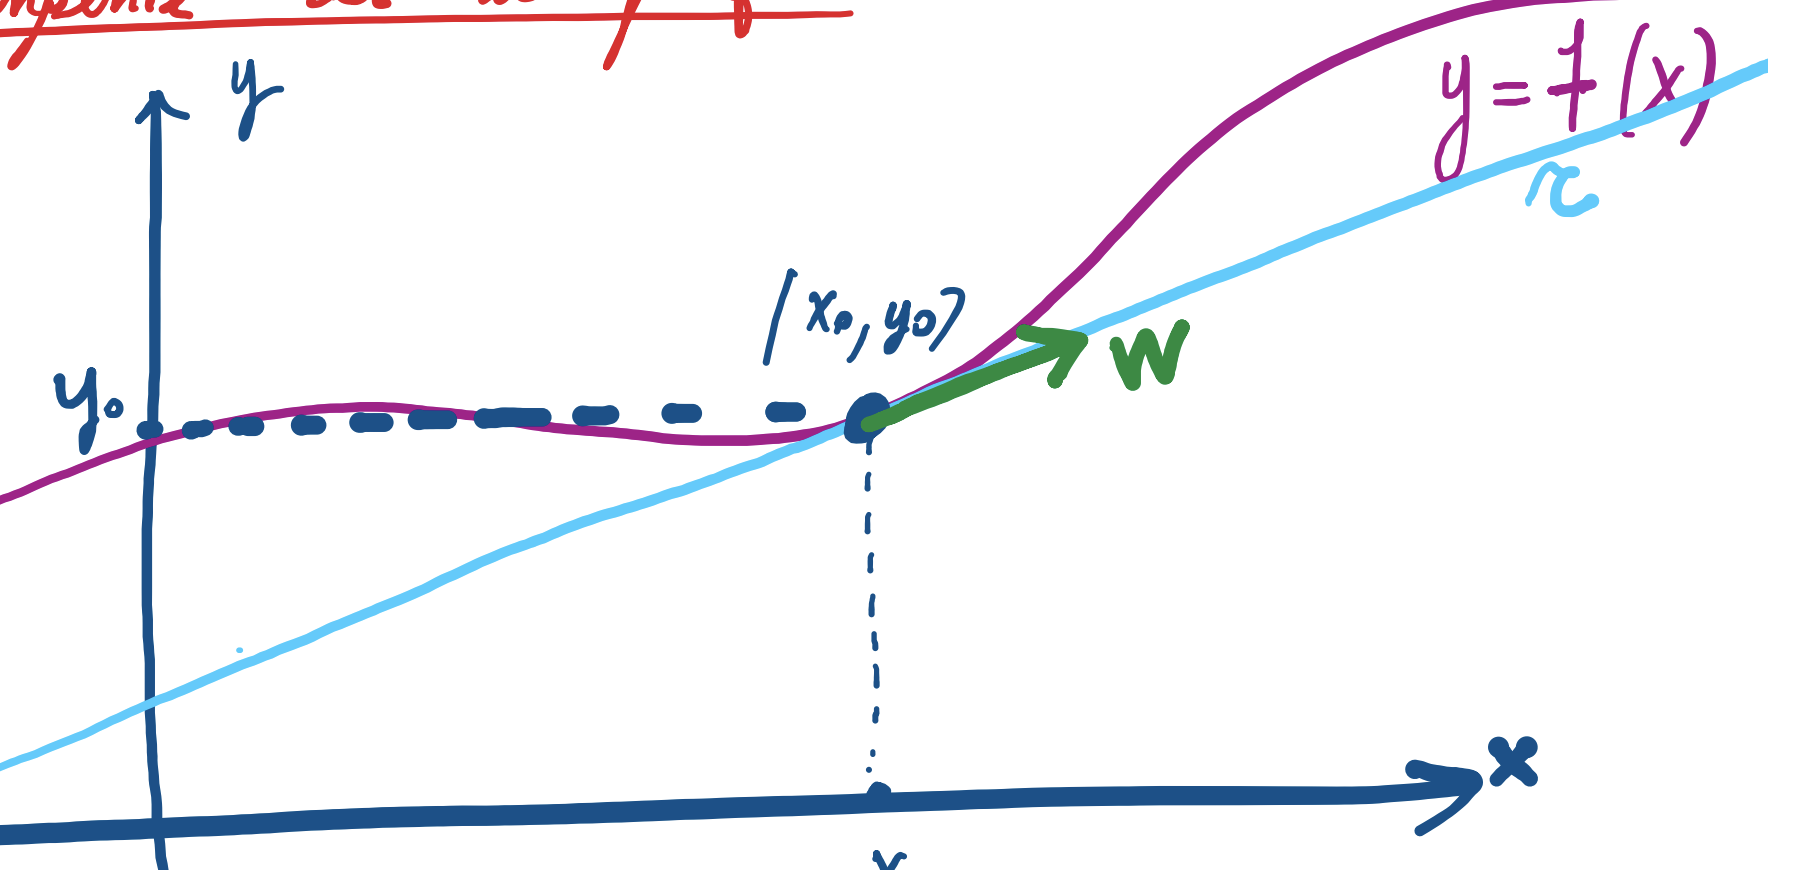
\includegraphics[width=5cm]{images/retta-tangente-in-R3.png}
\end{wrapfigure}
Il suo grafico $graf(f) \subset \mathbb{R}^2$. dato un $x_0 \in \mathbb{R}$ chiamo $y_0 = f(x_0)$ possiamo fare lo sviluppo di Taylor di f in $x_0$ di primo ordine, l'obbiettivo qui è scrivere l'equazione della retta che passa per $x_0, y_0$ tangente a $f$. Lo sviluppo è: $f(x) = f(x_0) + f'(x_0)(x-x_0) + o(x-x_0)$.\\ \\
Sappiamo che $y = f(x)$ ci da il grafico di $f$, quindi ci chiediamo $y = f(x_0) + f'(x_0)(x-x_0)$ che grafico sia. Possiamo vedere che:
\begin{enumerate}
    \item Come prima cosa si tratta di una retta perché $f'(x_0)x + y - f'(x_0)x_0 + f(x_0) = 0$.
    \item Poi osservo che questa retta passa per $(x_0, y_0)$, perché se sostituisco $x=x_0$ ho $y = f(x_0) = y_0$ che sta sul grafico di $f$.
    \item Inoltre grazie allo sviluppo di Taylor posso concludere che la differenza fra i due grafici $f(x) - f(x_0) - f'(x_0)(x-x_0) = o(x-x_0)$.
\end{enumerate}
Date tutte queste considerazioni possono concludere che $y=f(x_0) + f'(x_0)(x-x_0)$ è la retta tangente al grafico $y=f(x)$ in $(x_0, y_0)$. Proviamo ora a riscriverla nella forma $ax + by + c = 0$.
\[y - f(x_0) - f'(x_0)\cdot(x-x_0) = 0 \rightarrow y - f(x_0) f'(x_0)x + f'(x_0)x_0 = 0 \rightarrow -f'(x_0)x + y + f'(x_0)x_0 - f(x_0) = 0\]
Questa è la forma cartesiana della retta r dove $a = -f'(x_0)$ e $b = 1$.\\
$v = (a,b) = (-f'(x_0), 1)$ è perpendicolare a r $\Longrightarrow w = (1, f'(x_0))$ è vettore tangente ad r tale che $<v,w> = 0$. Abbiamo quindi il vettore $w = (1, f'(x_0)$ che è tangente alla retta, posso allora dimostrare che questa retta è tangente. Prima di tutto sappiamo che la retta tange al grafico di $f(x)$ in $(x_0, y_0)$ per definizione è la retta passante per il punto $(x_0, y_0)$ che ha coefficiente angolare $= f'(x_0)$.\\
La retta r di equazione $y - f'(x_0)x + f'(x_0)x_0 - f(x_0) = 0$ che ha come vettore tangente w ha come coefficiente angolare $f'(x_0)$. Ora metto insieme tutte le informazione:
\begin{itemize}
    \item La retta r passa per $(x_0, y_0)$.
    \item La retta r ha come coefficiente angolare $f'(x_0)$
\end{itemize}
Quindi possiamo vedere che r è la retta tangente a $y=f(x)$ nel punto $(x_0, y_0)$. Possiamo riscriverla nella seguente forma cartesiana:
\[y = f(x_0) + f'(x_0)(x-x_0)\]
Mentre la forma parametrica è la seguente.
\[r: \Bigg\{ \begin{pmatrix}x\\y\end{pmatrix} = \begin{pmatrix}x_0\\y_0\end{pmatrix} + t \begin{pmatrix}1\\f'(x_0)\end{pmatrix}\Bigg\}\]
In $\mathbb{R}^2$ una retta è descritta da una sola equazione perché in $\mathbb{R}^2$ ho due gradi di liberta che sono le due variabili mentre su una retta posso solo muovermi sulla retta.

\subsection{Spazio cartesiano in $\mathbb{R}^3$}
Nel caso ci trovassimo in un $\mathbb{R}^3$ abbiamo un vettore scritto come $v = (x_1, y_1, z_1)$. $\mathbb{R}^3$ ha 3 gradi di liberà (x,y,z) mentre la retta ha 1 grado di libertà quindi ci aspettiamo che per descrivere una retta in uno spazio sarà descritta in 2 equazioni perché dai 3 gradi ne devo vincolare 2.

\subsubsection{Retta passante per due punti}
\begin{wrapfigure}[6]{r}{5cm}
    \vspace{-15pt}
    \centering
    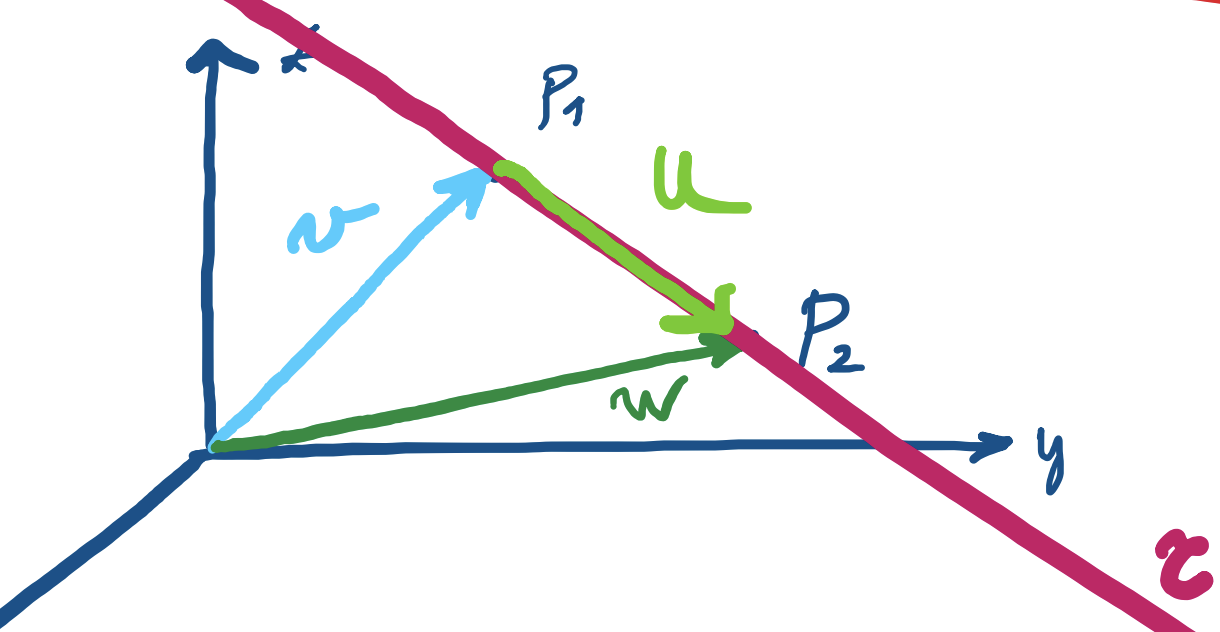
\includegraphics[width=4.2cm]{images/retta-passante-2-punti-R3.png}
\end{wrapfigure}
Una retta passante per 2 punti in $\mathbb{R}^3$ possiamo prendere due punti con i vettori associati $P_1 = (x_1, y_1, z_1)$ e $P_2 = (x_2, y_2, z_2) = w$, noi vogliamo scrivere l'equazione della retta che passa per $P_1, P_2$. 
Chiamiamo $u = w-v = (x_2 - x_1, y_2-y_1, z_2-z_1)$, ottengo la forma parametrica di r scrivendo r come:
\[r = \{P = v + tu \::\: t \in \mathbb{R}\} = \Bigg\{ \begin{pmatrix}x\\y\\z\end{pmatrix}\in \mathbb{R}^3 \::\: \begin{pmatrix}x\\y\\z\end{pmatrix} =  \begin{pmatrix}x_1\\y_1\\z_1\end{pmatrix} = t\begin{pmatrix}x_2 - x_1\\y_2 - y_1\\z_2 - z_1\end{pmatrix}\Bigg\}\]
La forma cartesiana di r invece la possiamo scrivere ricavando il paramento:
\[\begin{cases}x=x_1+t(x_2-x_1)\\y=y_1 +t(y_2 - y_1)\\z=z_1 + t(z_2-z_1)\end{cases} = \begin{cases}t = \frac{x-x_1}{x_2 - x_1}\\t = \frac{y-y_1}{y_2 - y_1}\\t=\frac{z-z_1}{z_2-z_1}\end{cases} = \begin{cases}\frac{x-x_1}{x_2-x_1} = \frac{y-y_1}{y_2-y_1}\\\frac{y-y_1}{y_2-y_1} = \frac{z-z_1}{z-z_2}\end{cases}\]

\vspace{20pt}
\subsubsection{Piano in $\mathbb{R}^3$ passante per 3 punti}
\begin{wrapfigure}[5]{l}{5cm}
    \vspace{-10pt}
    \centering
    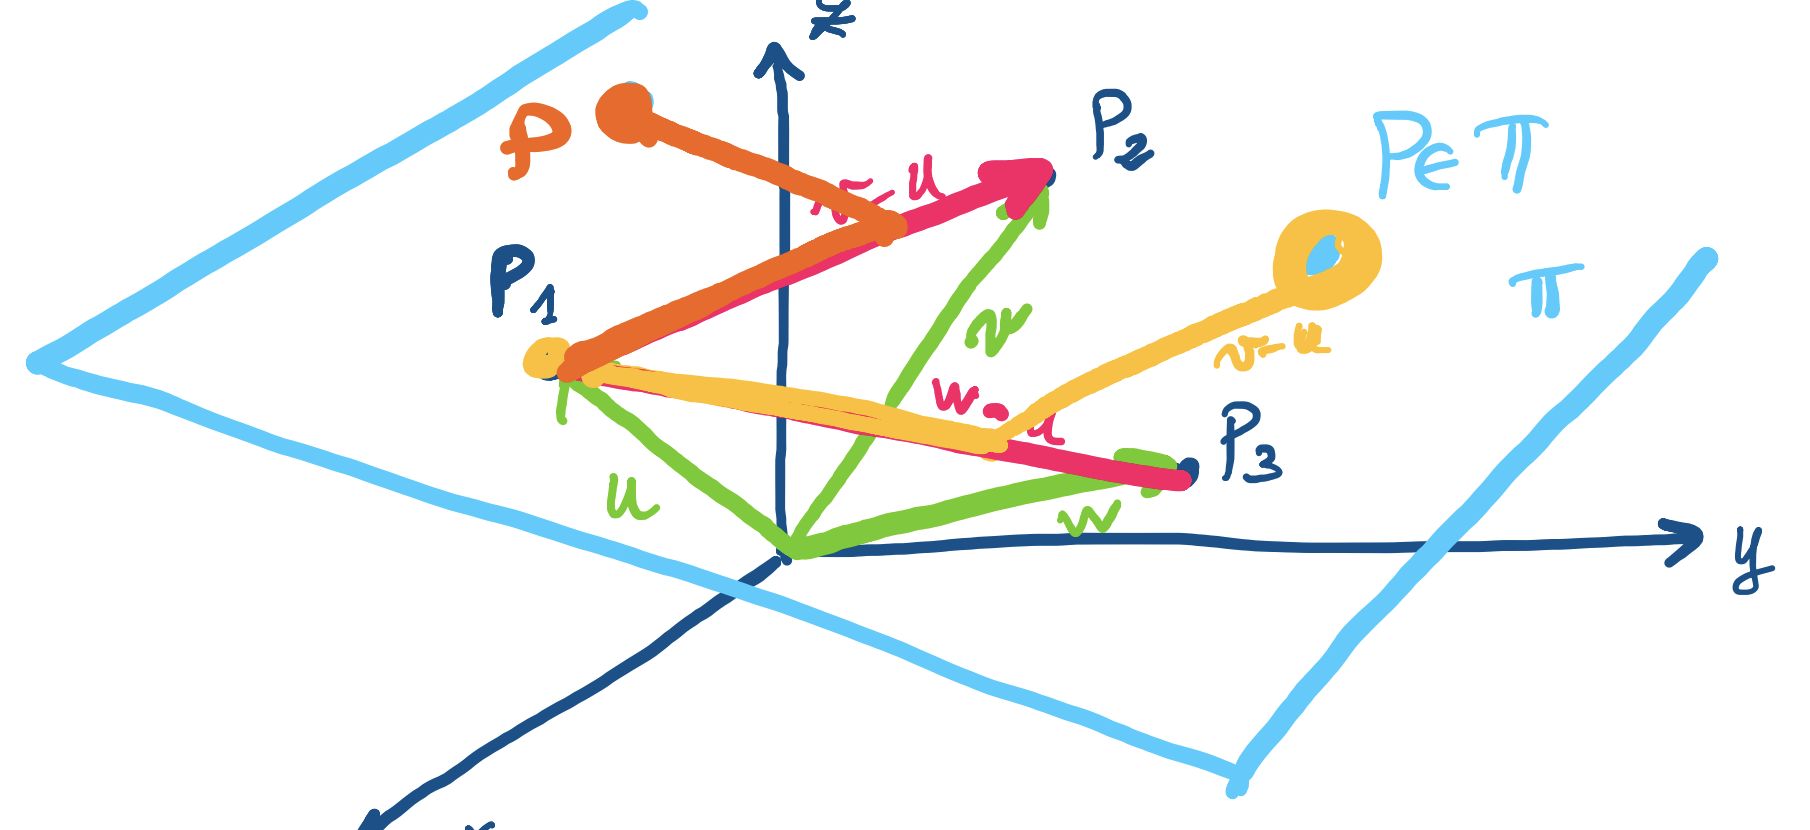
\includegraphics[width=4.5cm]{images/retta-passante-3-punti-R3.png}
\end{wrapfigure}
La prima cosa è scrivere l'equazione su $\mathbb{R}^3$ passante per 3 punti. Prendo innanzitutto 3 punti $P_1 = (x_1, y_1, z_1), P_2 = (x_2, y_2 z_2), P_3 = (x_3 y_3, z_3)$. Vediamo poi che in un piano ci sono 3 gradi di libertà, mentre nello spazio abbiamo 3 gradi di liberà, quindi ci aspettiamo 1 equazione lineare per definire un piano dello spazio. \\\\
Chiamiamo i vettori per i 3 punti $u = P_1, v = P_1, w = P_3$. Poi definiamo il piano per questi 3 punti che chiamiamo $\pi$, scriviamo poi:\\ $P_2 - P_1 = v-u = (x_1 - x_1, y_2 - y_1, z_2 - z_1)$ \hspace{.3cm} $P_3 - P_1 = w- u = (x_3 - x_1, y_3 - y_1, z_3 - z_1)$\\
La forma parametrica di $\pi$ può essere scritta come:
\[\pi = \Bigg\{\begin{pmatrix}x\\y\\z\end{pmatrix}\in \mathbb{R}^3 \::\: \begin{pmatrix}x\\y\\z\end{pmatrix} = P_1+t(v-u)+s(w-v) \::\: t,s \in \mathbb{R}\Bigg\} = \Bigg\{\begin{pmatrix}x\\y\\z\end{pmatrix} = \begin{pmatrix}x_1\\y_1\\z_1\end{pmatrix} + t\begin{pmatrix}x_2-x_1\\y_2-y_1\\z_2-z_1\end{pmatrix}+s\begin{pmatrix}x_3 - x_1\\y_3 -y_1\\z_3 - z_1\end{pmatrix}\Bigg\}\]
Se passo alla forma cartesiana vedo che l'equazione lineare che ottengo è una sola.
\[\begin{cases}x = x_1 + t(x_2 - x_1) + s(x_3 - x_1)\\ y = y_1 + t(y_2 - x_1) + s(y_3 - y_1)\\z = z_1 + t(z_2 - z_1) + s(z_3 - z_1)\end{cases} = \begin{cases}\frac{x - x_1}{x_2 - x_1} = t + s \frac{x_3 - x_1}{x_2 - x_1}\\ \frac{y-y_1}{y_2-y_1} = t + s\frac{y_3-y_1}{y_2-y_1}\\ \frac{z-z_1}{z_2-z_1} = t + s\frac{(z_3 - z_1)}{z_2 - z_1}\end{cases} = \text{1°eq - 2°eq}  = \]
\[= \begin{cases}\frac{x-x_1}{x_2-x_1} - \frac{y-y_1}{y_2-y_1} = s(\frac{x_3-x_1}{x_2-x_1} - \frac{y_3 - y_1}{y_2-y_1})\\\frac{x-x_1}{x_2-x_1} - \frac{z - z_1}{z_2-z_1} = s(\frac{x_3-x_1}{x_2-x_1} - \frac{z_3 - z_1}{z_2-z_1})\end{cases} = \begin{cases}s = \frac{(\frac{x-x_1}{x_2 - x_1} - \frac{y-y_1}{y_2-y_1})}{(\frac{x_3-x_1}{x_2-x_1} - \frac{y_3 - y_1}{y_2 - y_1})}\\s = \frac{(\frac{x-x_1}{x_2-x_1} - \frac{z -z_1}{z_2 - z_1})}{(\frac{x_3 - x_1}{x_2 - x_1} - \frac{z_3-z_1}{z_2-z_1})}\end{cases} = \frac{\frac{x-x_1}{x_2-x_1} - \frac{y - y_1}{y_2-y_1}}{\frac{x_3-x_1}{x_2-x_1} - \frac{y_3-y_1}{y_2-y_1}} = \frac{\frac{x-x_1}{x_2-x_1} - \frac{z-z_1}{z_2-z_2}}{\frac{x_3 - x_1}{x_2-x_1} - \frac{z_3-z_1}{z_2-z_1}}\]
Questa è 1 equazione linerare che è l'equazione cartesiana di $\pi$ piano passante per $P_1, P_2, P_3$.

\subsection{Disegno di insiemi nel piano}
Il primo obbiettivo e dunque quello di disegnare insiemi di $\mathbb{R}^2$ descritti da equazioni e o disequazioni. Per farlo vediamo alcuni esempi per vedere come visualizzare nel piano.

\begin{example}\label{ess-1}
Prendiamo $x, y \in \mathbb{R}$, e disegnammo $\{(x,y) \in \mathbb{R}^2 \::\: (x+y) \ge1 0\}$. Sappiamo che $x+y \geq 0 \Longleftrightarrow y \geq -x$ e questa è una retta della forma $y + y = 0$ ma noi prendiamo solo i punti sopra visto che usiamo un maggiore uguale. 
\end{example}

\begin{example}\label{ess-2}
Disegnammo $\{(x,y) \in \mathbb{R}^2 \::\: x-y \leq 0 \}$, quindi abbiamo $y = x$ e visto che abbiamo il minore uguale prendiamo tutti i punti sotto.
\end{example}

\begin{example}\label{ess-3}
Ora prendiamo $\{(x,y) \in \mathbb{R}^2 \:\: 3 \leq x+y \leq 5\}$, in questo caso però ci sono due condizioni che devono essere verificate contemporaneamente quindi mettiamo tutto come un sistema:\\
$\begin{cases}x+y \geq 3 \\ x+y \leq 5\end{cases} = \begin{cases}y \geq 3-x & \text{ Si in individua una retta della forma } y=3-x \\ y \leq 5-x & \text{ Si in individua una retta della forma } y=5-x\end{cases}$\\
Disegniamo queste due rette e poi prendiamo i punti compresi fra entrambe. La soluzione è dunque l'intersezione fra i due insiemi.
\end{example}

\begin{figure}[h!]
\centering
\begin{subfigure}{.3\textwidth}
    \centering
    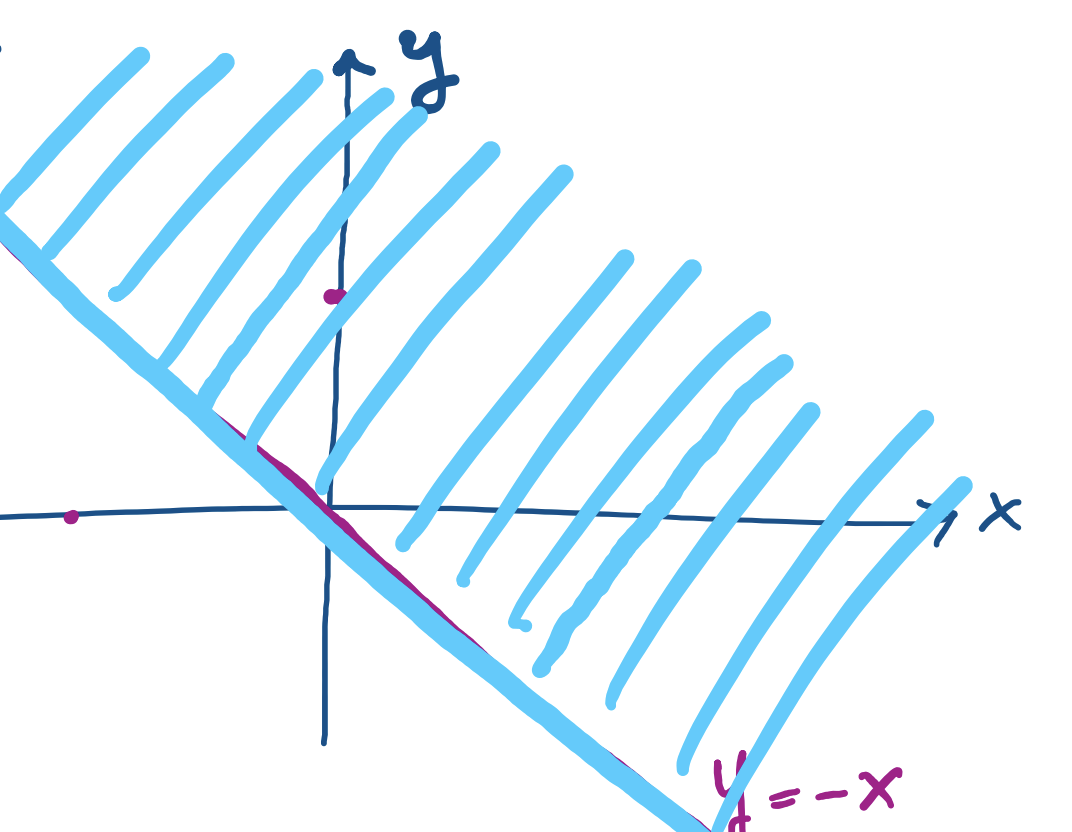
\includegraphics[width=4cm]{images/disegno-R3-ess1.png}
    \caption{Esempio \ref{ess-1}}
\end{subfigure}
\begin{subfigure}{.3\textwidth}
    \centering
    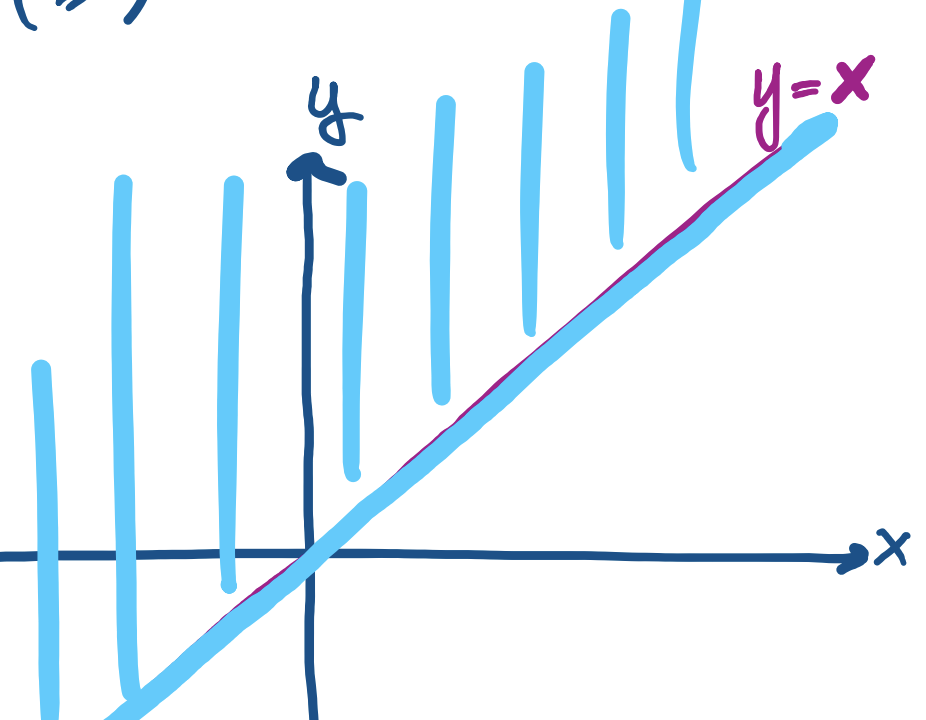
\includegraphics[width=4cm]{images/disegno-R3-ess2.png}
    \caption{Esempio \ref{ess-2}}
\end{subfigure}
\begin{subfigure}{.3\textwidth}
    \centering
    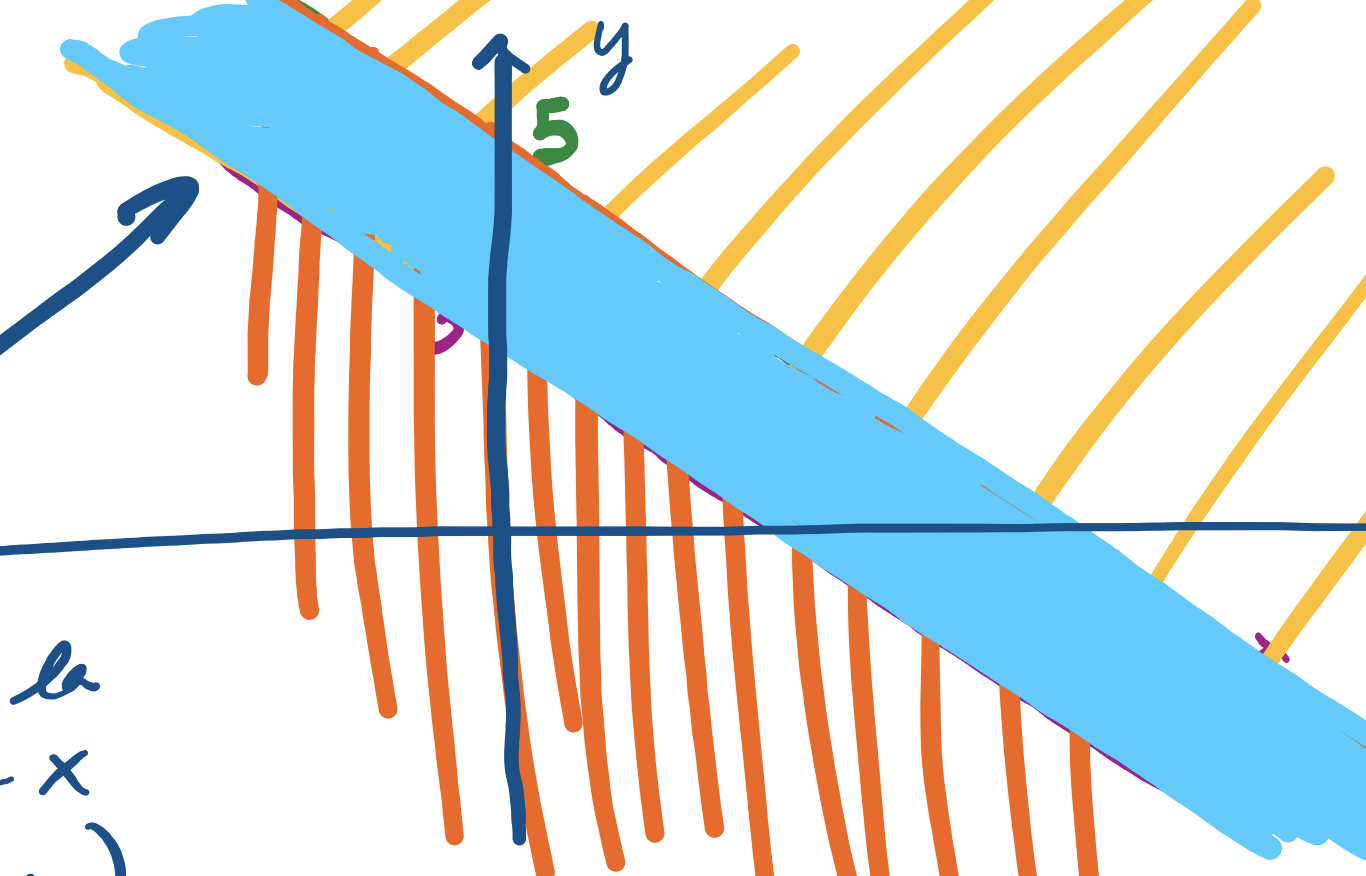
\includegraphics[width=4cm]{images/disegno-R3-ess3.png}
    \caption{Esempio \ref{ess-3}}
\end{subfigure}
\end{figure}

\begin{example}\label{ess-4}
Consideriamo $\{(x,y) \in \mathbb{R}^2 \::\: x \cdot y \geq 0\}$ affinché il prodotto di $x, y$ si maggiore e uguale di zero dobbiamo vedere i due casi mettendoli a sistema:\\
$\begin{cases}x \geq 0 \\ y \geq 0\end{cases}$ e $\begin{cases}x \leq 0 \\ y \leq 0\end{cases}$
Infatti affinché $x \cdot y \geq 0$ x ed y devono essere concordi. Quindi prendiamo le parti del piano che soddisfano la proprietà di avere x ed y concordi.
\end{example}

\begin{example}\label{ess-5}
Dato $\{(x,y) \in \mathbb{R}^2 \::\: x^2 - x \geq 0\}$. Sappiamo che $x^2 - x \geq 0$ è uguale a $x(x-0) \geq 0$ e questa equazione perché sia maggiore o uguale a 0:
$\begin{cases}x \geq 0 \\ x \geq 1\end{cases}$ o $\begin{cases}x \leq 0 \\ x \leq 1\end{cases}$ quindi $x \geq 0$ o $x \leq 0$.
\end{example}

\begin{example}\label{ess-6}
Consideriamo $\{(x,y) \in \mathbb{R}^2 \::\: x^2 + y^2 \geq 8\}$. Se abbiamo un punto $(x,y)$ e consideriamo $x^2 + y^2$ sappiamo che $d((x,y), (0,0)) = |(x+y) - (0,0)| = |(x,y)| = \sqrt{x^2 + y^2}$. Quindi abbiamo che se $x^2 + y?^2 \geq 8 \Longleftrightarrow$ distanza di $(x,y)$ dall'origine maggiore o uguale a $\sqrt{8}$.
\end{example}

\begin{example}\label{ess-7}
In modo analogo all'esempio prima se consideriamo $\{(x,y) \in \mathbb{R}^2 \::\: x^2+y^2 \leq 8\}$ abbiamo tutti i punti interni alla circonferenza con la circonferenza inclusa.
\end{example}

\begin{figure}[h!]
\centering
\begin{subfigure}{.23\textwidth}
    \centering
    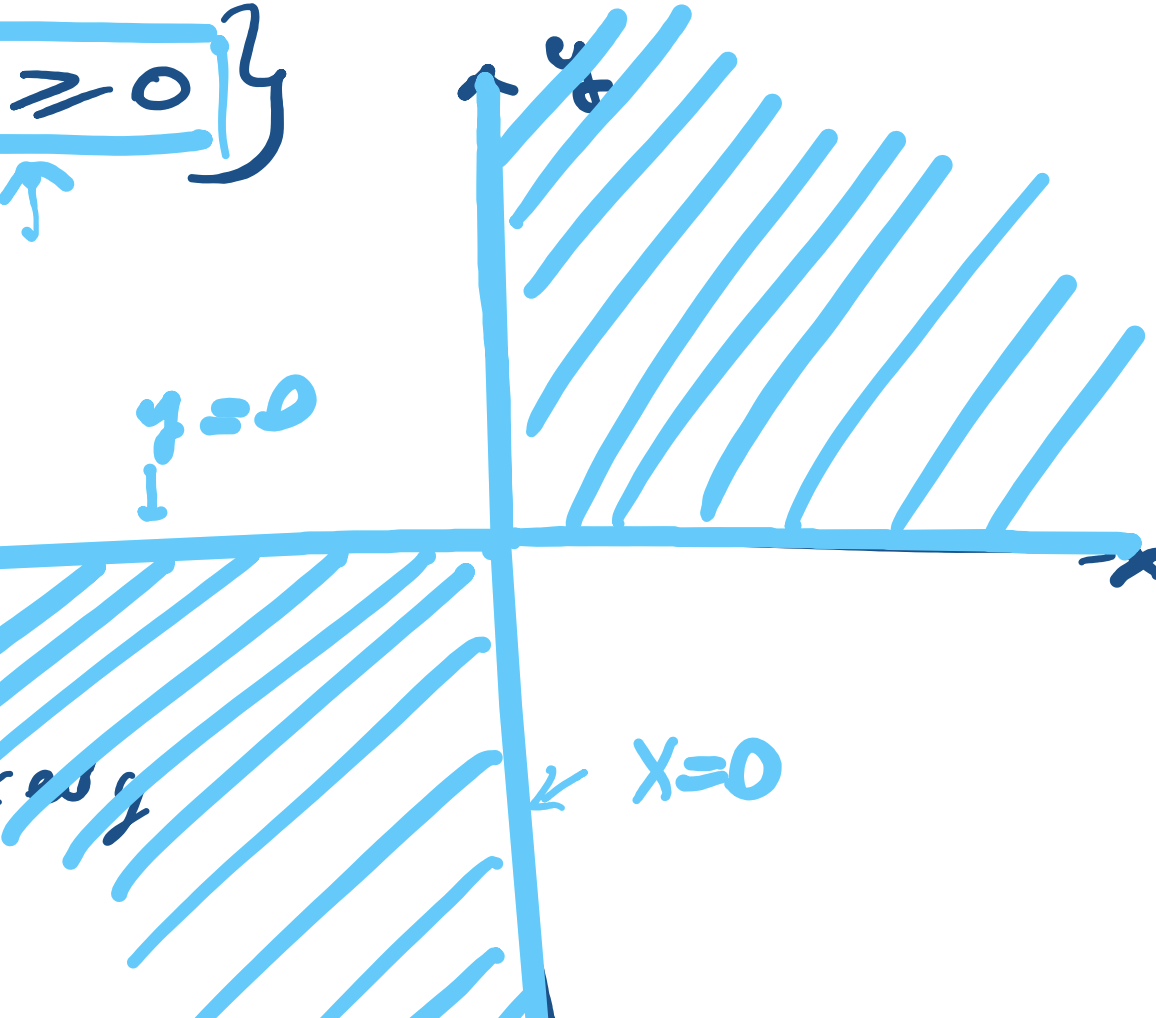
\includegraphics[width=3cm]{images/disegno-R3-ess4.png}
    \caption{Esempio \ref{ess-4}}
\end{subfigure}
\begin{subfigure}{.23\textwidth}
    \centering
    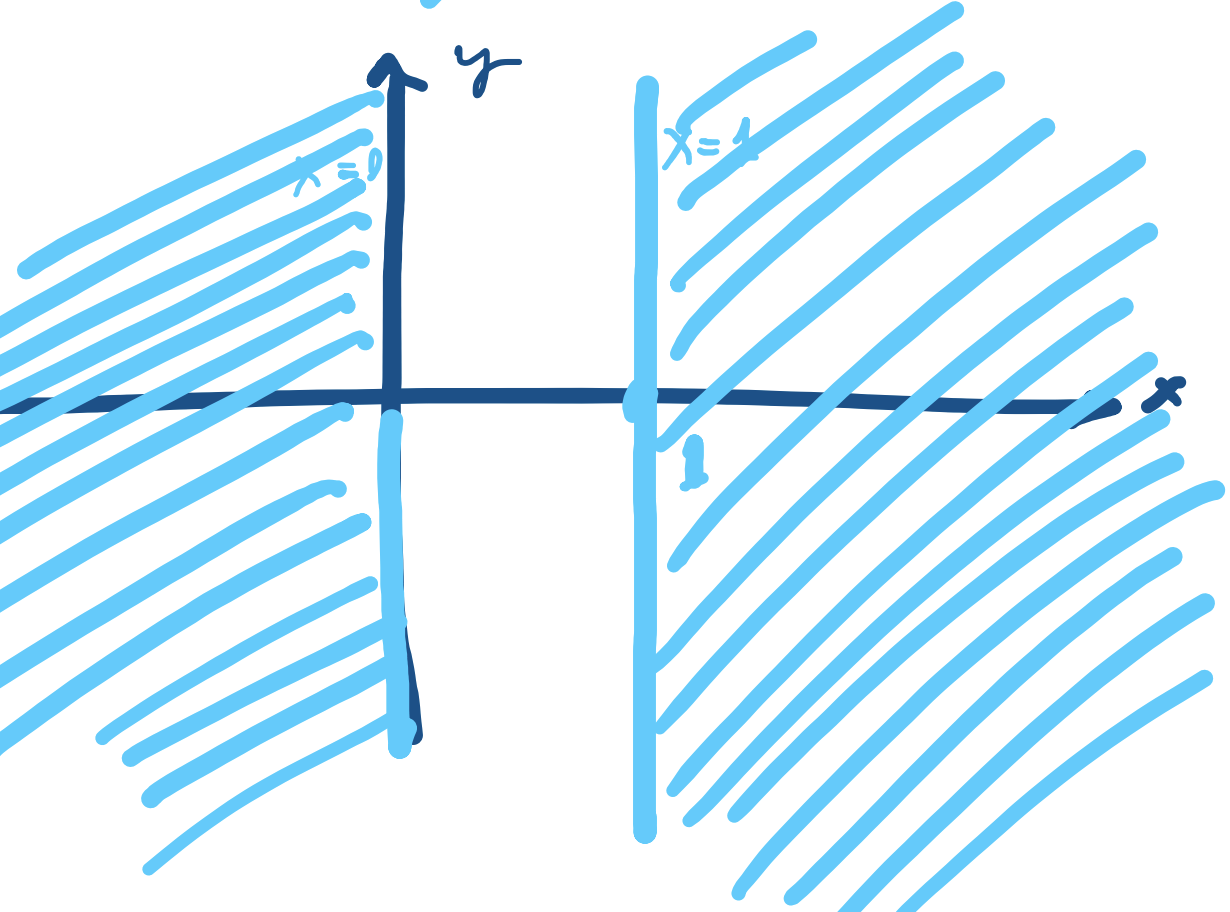
\includegraphics[width=3cm]{images/disegno-R3-ess5.png}
    \caption{Esempio \ref{ess-5}}
\end{subfigure}
\begin{subfigure}{.23\textwidth}
    \centering
    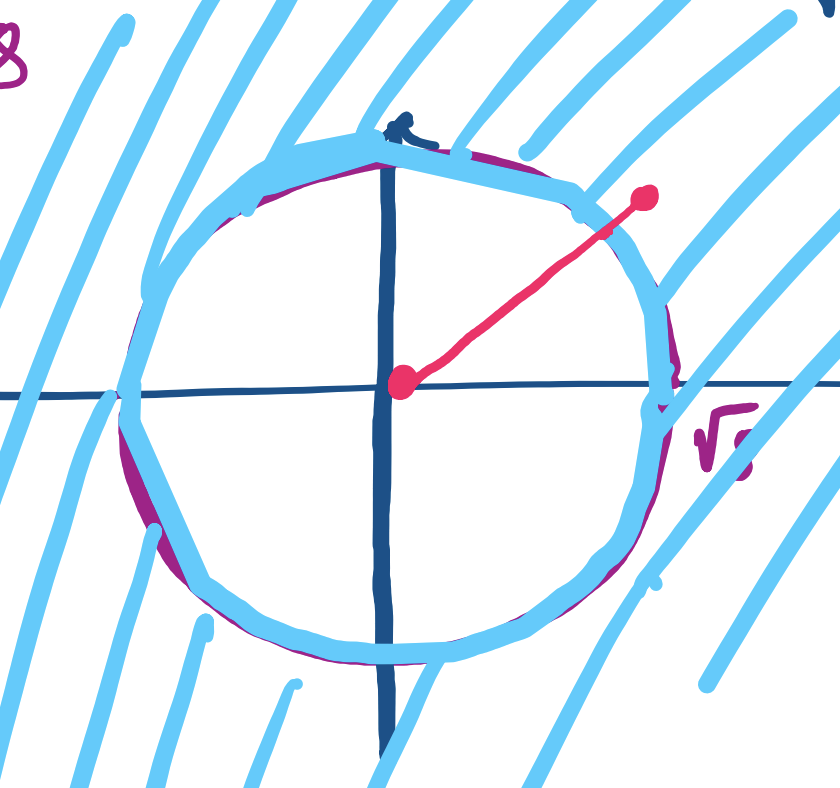
\includegraphics[width=3cm]{images/disegno-R3-ess6.png}
    \caption{Esempio \ref{ess-6}}
\end{subfigure}
\begin{subfigure}{.23\textwidth}
    \centering
    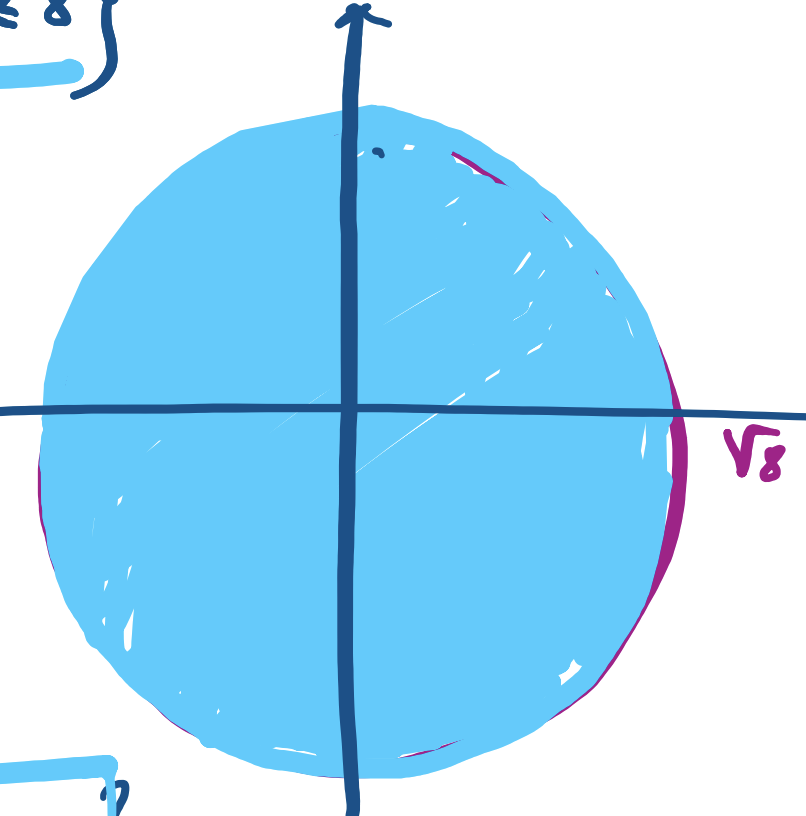
\includegraphics[width=3cm]{images/disegno-R3-ess7.png}
    \caption{Esempio \ref{ess-7}}
\end{subfigure}
\end{figure}

\begin{example}\label{ess-8}
Consideriamo l'insieme dei punti $\{(x,y) \in \mathbb{R^2} \::\: y \leq x^2 - x\}$. Sappiamo che $y = x^2 -x$ descrive una parabola con concavità verso l'alto e toccando l'asse x in 0 e 1. Questa equazione individua tutti i punti che stanno sotto la parabola inclusa appunto la parabola.
\end{example}

\begin{example}\label{ess-10}
Se andassi a considerare invece $\{(x,y) \in \mathbb{R^2} \::\: x^2 - x \leq y \leq 0\}$ come nell'esempio di prima si crea un parabola concava verso l'alto ma in questo caso dobbiamo mettere a sistema due condizioni:\\
$\begin{cases}y \geq x^2 - x & \text{ sopra la parabola } \\ y \leq 0 & \text{ sotto l'asse x }\end{cases}$
\end{example}

\begin{example}\label{ess-11}
Se andiamo a considerare $\{(x,y) \in \mathbb{R}^2 \::\:  |x| \leq 5\}$. Abbiamo che, essendo un valore assoluto, $-5 \leq x \leq 5$. Quindi andiamo a considerare che abbiamo la parte compreso fra le rette $x = -5$ e $x = 5$ comprese.\\
Mq in generale $\{|x| \leq A\}$ con A un generico numero, ha come soluzioni:
\begin{itemize}
    \item Insieme vuoto se $A < 0$.
    \item Abbiamo poi $x = 0$ se $A = 0$.
    \item Ed in fine $-A \leq x \leq A$ se $A > 0$
\end{itemize}
Analogamente la disequazione $|x| \geq A$ (con $x \in \mathbb{R}$, i valore assoluto) ha come soluzioni:
\begin{itemize}
    \item Tutto $\mathbb{R}$ se $A \leq 0$.
    \item Invece abbiamo $x \leq -A$ e $x \geq A$ se $A > 0$.
\end{itemize}
\end{example}

\begin{example}\label{ess-12}
Se ci troviamo allora a descrivere $\{(x,y) \in \mathbb{R}^2 \::\: |x| \leq 5, |y| \leq 3\}$. Siccome sono nel caso in cui abbiamo due numeri positivi abbiamo:\\
Primo caso $|x| \leq 5 \Longleftrightarrow -5 \leq x \leq 5$ e nel secondo caso $|y| \leq 3 \Longleftrightarrow -3 \leq y \leq 3$, quindi combinando tutti questi casti risulta un area specifica.
\end{example}

\begin{figure}[h!]
\centering
\begin{subfigure}{.23\textwidth}
    \centering
    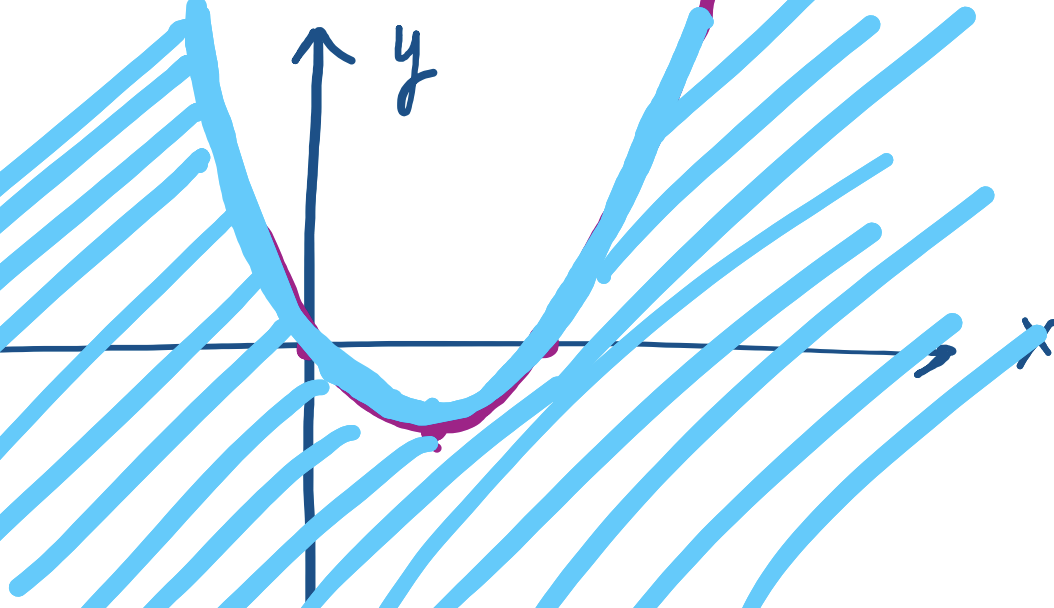
\includegraphics[width=3cm]{images/disegno-R3-ess8.png}
    \caption{Esempio \ref{ess-4}}
\end{subfigure}
\begin{subfigure}{.23\textwidth}
    \centering
    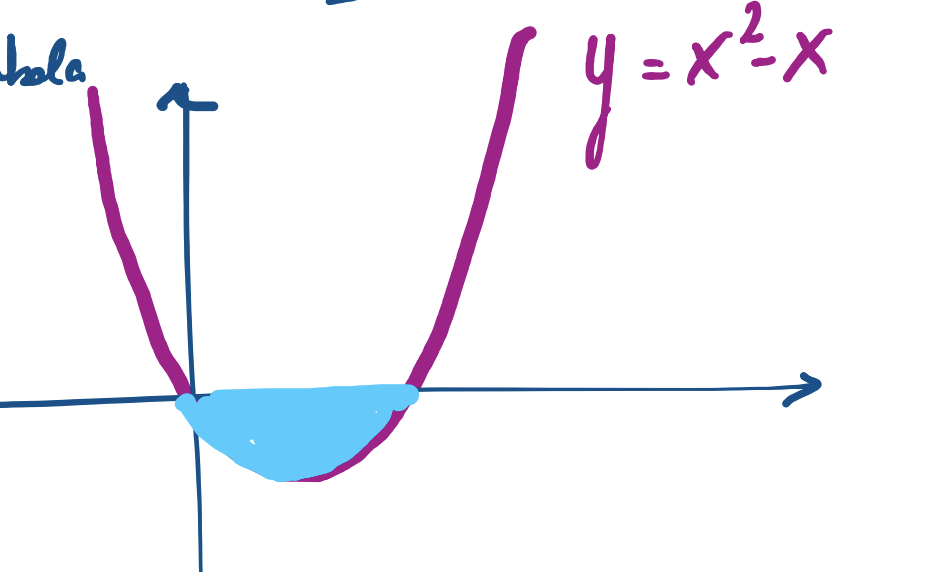
\includegraphics[width=3cm]{images/disegno-R3-ess10.png}
    \caption{Esempio \ref{ess-5}}
\end{subfigure}
\begin{subfigure}{.23\textwidth}
    \centering
    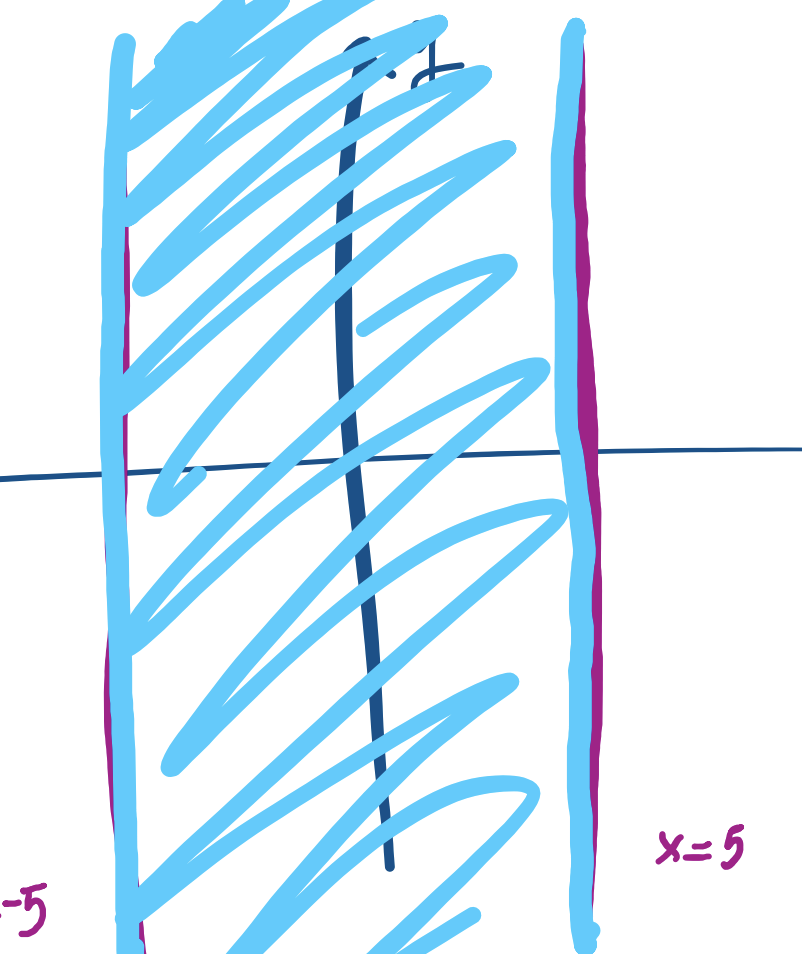
\includegraphics[width=3cm]{images/disegno-R3-ess11.png}
    \caption{Esempio \ref{ess-6}}
\end{subfigure}
\begin{subfigure}{.23\textwidth}
    \centering
    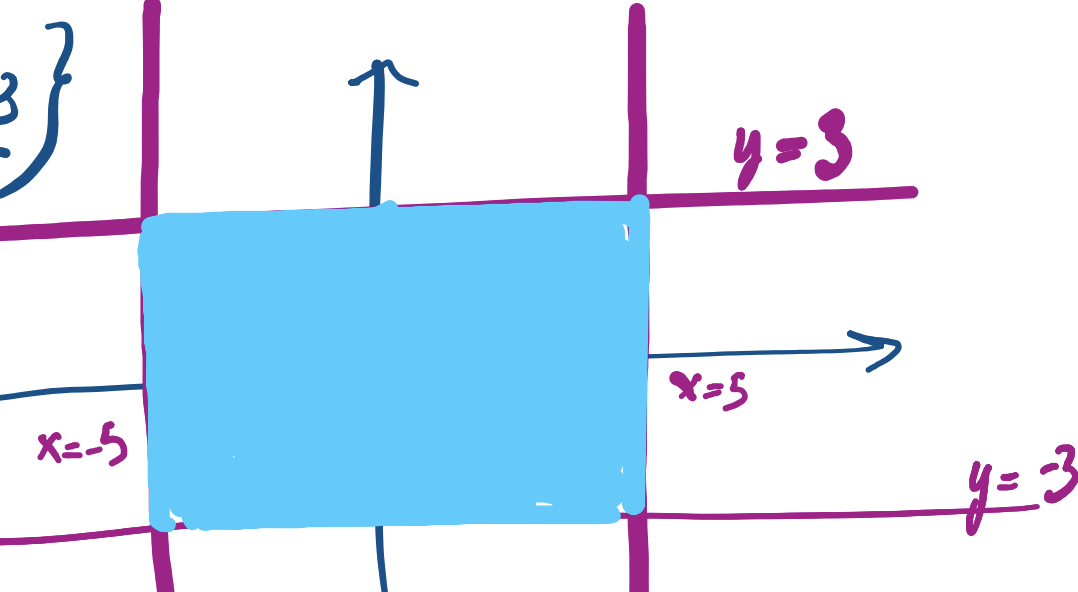
\includegraphics[width=3cm]{images/disegno-R3-ess12.png}
    \caption{Esempio \ref{ess-7}}
\end{subfigure}
\end{figure}

\subsection{Curva nel piano e nello spazio}
Noi conosciamo come disegnare parabole, iperbole rette ma volgiamo poter definire anche un oggetto più generico.
\begin{definition}[Curva nel piano]
Una \textbf{curva nel piano} è una funzione $\gamma: I \to \mathbb{R}^2$ con $I \subseteq \mathbb{R}$.
\end{definition}
\hspace{-15pt}Per noi possiamo avere sia $I = (a,b)$ intervallo aperto che $I = [a,b]$ intervallo chiuso. Se $I = [a,b]$ quindi intervallo chiuso allora possiamo definire una curva chiusa.

\begin{definition}[Curva chiusa]
Dato un $I = [a,b]$, una $\gamma: I \to \mathbb{R}^2$ si dice \textbf{curva chiusa} se $\gamma(a) = \gamma(b)$ (per farlo sostituisco gli estremi nella funzione $\gamma$).
\end{definition}

\begin{note}
Notare che la funzione che abbiamo a valori in $\mathbb{R}^2$, $\gamma: I \to \mathbb{R}^2$, indico utilizzando la seguente notazioni, chiamo $t \in I$ e $\gamma(t) = (x(t), y(t)) \in \mathbb{R}^2$.
\end{note}

\begin{example}
$\gamma(t) = (t^2 + 1, 3t -2)$, con $t \in [0,3]$ è una curva che ha come intervallo $[a,]b = [0,3]$ e le componenti sono $x(t) = t^2+1, y(t) = 3t-2$ che sono due funzioni in t. Per ogni punto $t \subseteq [0,3]$ la curva $\gamma$. individua un punto del piano. Per esempio $t = 0 \to \gamma(0) = (1,-2)$ mentre $t = 3 \to \gamma(3) = (10,7)$.
\end{example}
\hspace{-15pt}Con una curva sto rappresentano un punto che si muove nel piano, perché il paramento t lo posso interpretarlo come tempo quindi $\gamma(t)$ mi dice in che punto si trova la mia curva al tempo t.

\begin{definition}[Curva nello spazio]
Una \textbf{curva nello spazio} posso definirla come una funzione $\gamma: I \to \mathbb{R}^3$ con $I \subset \mathbb{R}$
\end{definition}

\begin{example}
Se prendiamo $\gamma(t) = (t^2, \sin{t}, e^t)$, $t \in [-1, 1]$ è un curva nello spazio. Vediamo che questa funzione prende 3 variabili che saranno 3 funzioni, $\gamma(t) = (x(t), y(t), z(t))$, $x: I\to \mathbb{R}, y: I\to \mathbb{R}, <: I\to \mathbb{R}$.
\end{example}

\begin{definition}[Curva semplice]
Una curva si dice \textbf{semplice} se "non ritorna mai su se stessa" (tranne al massimo $\gamma(a) = \gamma(b)$ cioè agli estremi può tornare su se stessa ma non in altri punti).
\end{definition}

\begin{figure}[h!]
\centering
\begin{subfigure}{.3\textwidth}
    \centering
    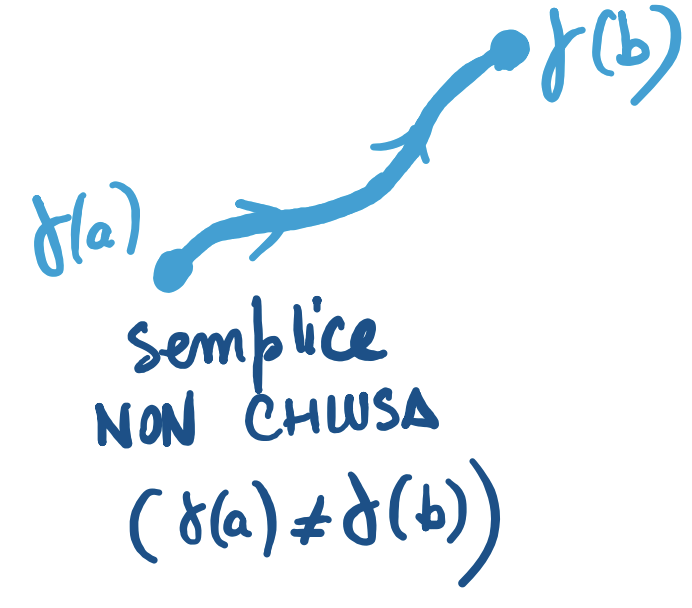
\includegraphics[width=3.2cm]{images/curva-semplice-non-chiusa.png}
    \caption{Esempio \ref{ess-4}}
\end{subfigure}
\begin{subfigure}{.3\textwidth}
    \centering
    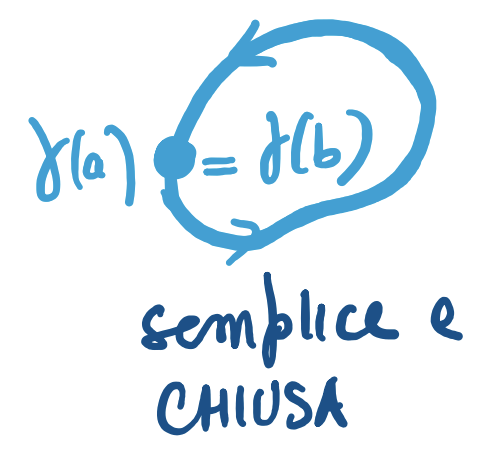
\includegraphics[width=3.2cm]{images/semplice-chiusa.png}
    \caption{Esempio \ref{ess-5}}
\end{subfigure}
\begin{subfigure}{.3\textwidth}
    \centering
    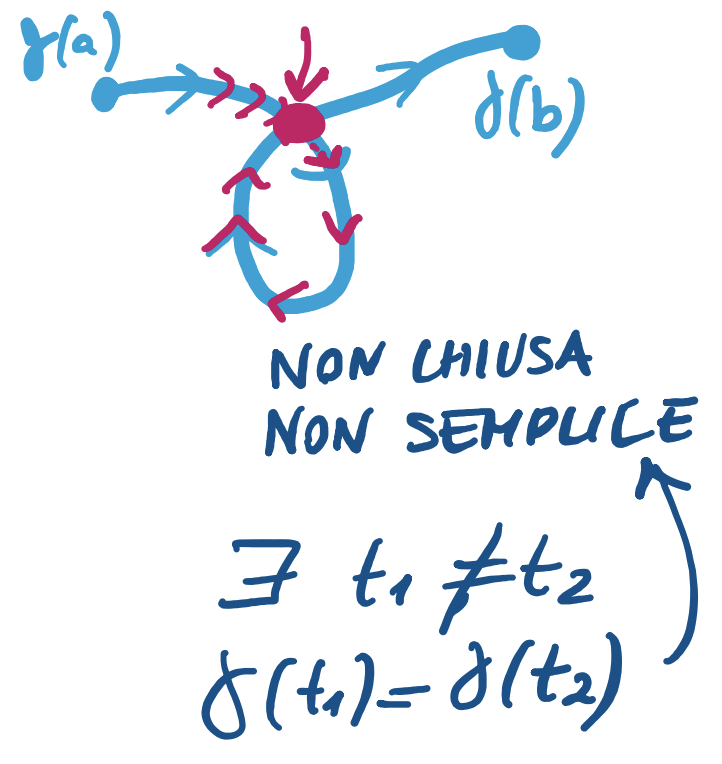
\includegraphics[width=3.2cm]{images/non-chiusa-non-semplice.png}
    \caption{Esempio \ref{ess-6}}
\end{subfigure}
\begin{subfigure}{.5\textwidth}
    \centering
    \vspace{20pt}
    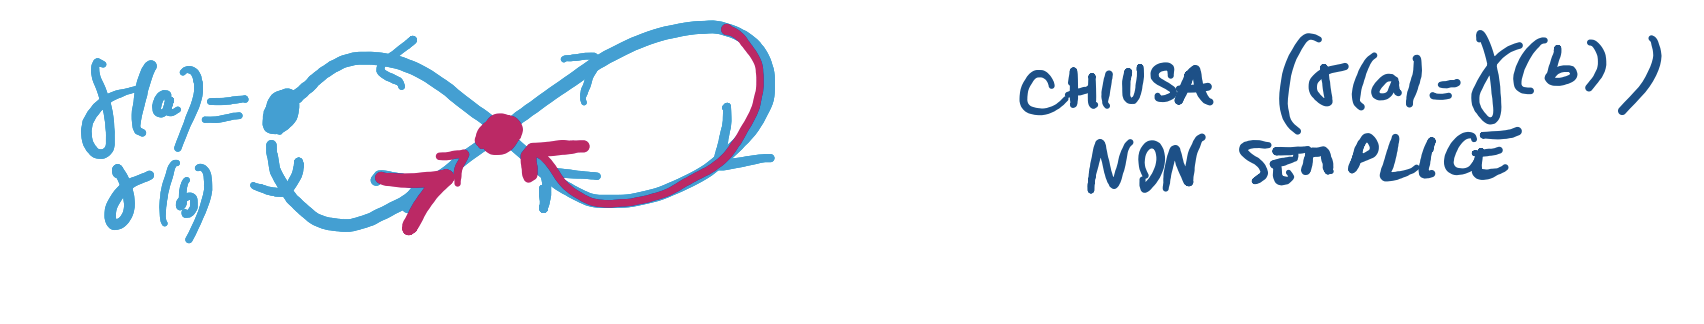
\includegraphics[width=10cm]{images/chiusa-non-semplice.png}
    \caption{Esempio \ref{ess-7}}
\end{subfigure}
\end{figure}

\begin{definition}[Sostegno di una curva]
Si dice \textbf{sostegno} di una curva l'immagine della curva stessa, cioè la traiettoria percorsa dal punto. 
\end{definition}
\hspace{-15pt}Per esempio possiamo avere $\gamma: [a,b] \to \mathbb{R}^2$, l'immagine $\gamma([a,b]) \subseteq \mathbb{R}^2$, ci darà quini un sottoinsieme. Se poi t lo consideriamo come il tempo allora $\gamma(t)$ punto in $\mathbb{R}^2$ dove si trova la curva al punto t.

\begin{definition}[Vettore tangente alla curva]
Sia $\gamma: I \to \mathbb{R}^2$ (o $\mathbb{R}^2$) con $I$ intervallo $\subset \mathbb{R}$. Si dice \textbf{vettore tangente} alla curva il vettore $\gamma'(t) = (x'(t), y'(t))$, assumendo che $x'(t), y'(t)$ esistano.
\end{definition}

\begin{observation}
$x: \mathbb{R} \to \mathbb{R}$, $y: \mathbb{R} \to \mathbb{R}$, abbiamo che $x'(t), y'(t)$ le sappiamo calcolare, quindi possiamo definire il vettore tangente.
\end{observation}

\begin{definition}[Retta tangente ad una curva]
La \textbf{retta tangente} ad una curva in un punto è la retta che passa per quel punto ed ha come direzione il vettore tangente alla curva in quel punto stesso.
\end{definition}

\vspace{50pt}
\begin{example}
Prendiamo la curva $\gamma(t) = (\sin{t}, \cos{t})$con $t \in [0,2\pi]$, $\gamma: [0,2\pi] \to \mathbb{R}^2$ e $\gamma(t) = (x(t), y(t))$ con $x(t) = \cos{t}$ e $y(t) = \sin(t)$.
\end{example}
\begin{wrapfigure}[10]{r}{5cm}
    \vspace{-10pt}
    \centering
    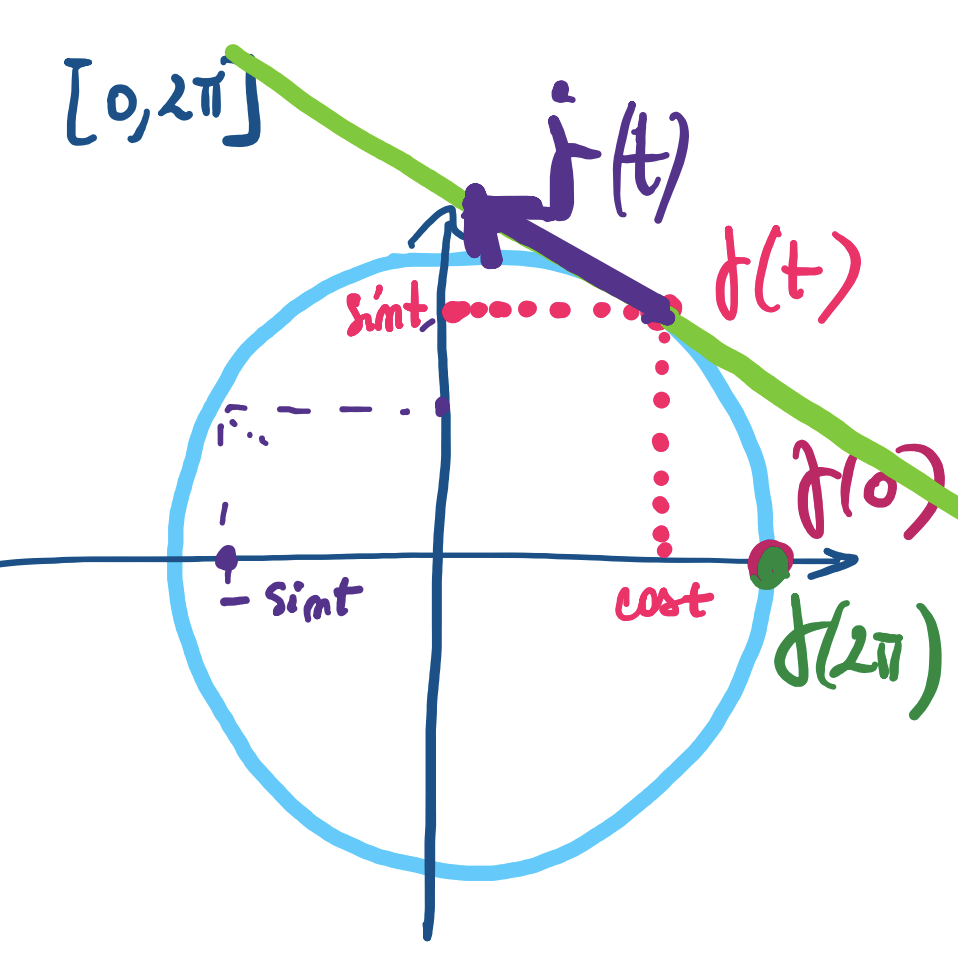
\includegraphics[width=4cm]{images/ess-curva-piano.png}
\end{wrapfigure}
 Se facciamo $x^2(t) + y^2(t) = \cos{t}^2 + \sin{t}^2 = 1 \forall \: t \in [0, 2\pi]$ e quindi $x^2(t) + y^2(t) = 1$. Il sostegno di $\gamma$ è la circonferenza (di $\mathbb{R}^2$) di equazioni $x^2 + y^2 = 1$ perché $\forall \: t \in [0,2\pi] \gamma(t) \in \{(x,y) \in \mathbb{R}^2 \::\: x^2+y^2 = 1\}$.\\
Il vettore tangente invece sarà $\mathring{E}(t) = (\mathring{x}(t), \mathring{y}(t)) = (-\sin{t}, \cos{t})$, se per esempio guardiamo il punto iniziale $\gamma(0) = (\cos{0}, \sin{0}) = (1,0)$ con $\gamma: [0,2\pi]$, mente se prendo il punto finale della traiettoria $\gamma(2\pi) = (\cos{2\pi}, \sin{2\pi}) = (1,0)$ e quindi ho $\gamma(0) = \gamma(2\pi)$ e quindi ho una curva chiusa.\\
La retta tangente nel punto t a $\gamma(t)$ la scrivo come: $r: \gamma(t) + s\mathring{\gamma(t)}$ che è la forma parametrica.

\begin{example}
Prendiamo la curva $\gamma(t) = (t, t^2+t)$ con $t \in [-1,2]$, abbiamo dunque che $x(t) = t$ e $y(t) = t^2 + t$. La curva percorre il tratto della parabole $y= x^2 + x$ però con $x \in [-1,2]$.
\end{example}
\begin{wrapfigure}[6]{r}{5cm}
    \vspace{-15pt}
    \centering
    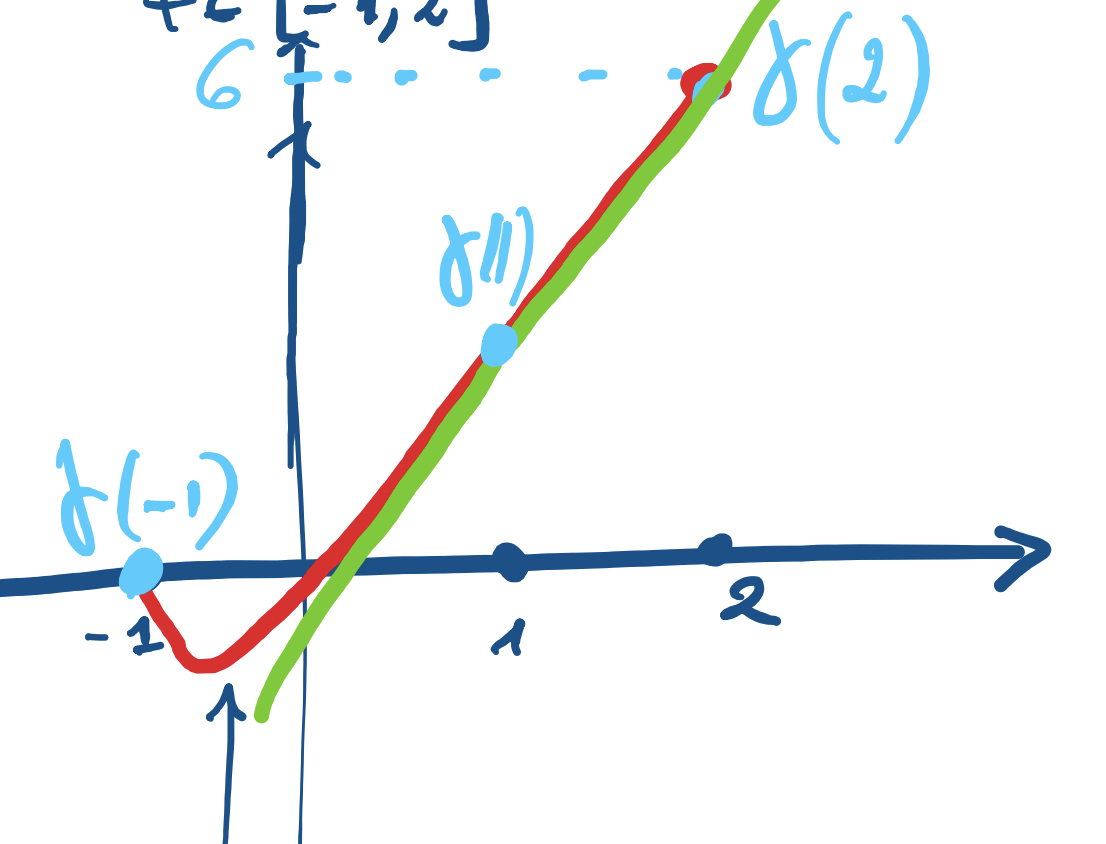
\includegraphics[width=4cm]{images/ess-curva-piano-2.png}
\end{wrapfigure}
Se prendiamo per esempio $\gamma(-1) = (1, 0)$, mentre $\gamma(2) = (2,6)$.\\
Proviamo a calcolare la retta tangente nel punto corrispondente a $t=1$, $\gamma(1) = (1,2)$ e $\gamma'(t) = (1, 2t+1)$ quindi $\gamma'(1) = (1,3)$, la retta tangente nel punto $\gamma(1) =$ la retta che passa per $\gamma(1) = (1,2)$ con direzione (1,3), al forma parametrica e dunque $(1,2) + s(1,3)$ con $s \in \mathbb{R}$. Vediamo che la curva è semplice ma non è chiusa.

\subsection{Funzioni di più variabili}
Fin ora abbiamo visto funzioni $f: \mathbb{R} \to \mathbb{R}$ o $f: A \to \mathbb{R}$ con $A \subseteq \mathbb{R}$. Mentre nell'analisi in più variabili avremo funzioni del tipo $f: \mathbb{R}^2 \to \mathbb{R}$, $f: \mathbb{R}^2 \to \mathbb{R}$ o più genericamente $f: \mathbb{R}^n \to \mathbb{R}$, queste funzioni posso anche essere $f: \Omega \to \mathbb{R}, \Omega \subseteq \mathbb{R}^n$.

\begin{definition}[Funzione, dominio, codominio]
Una \textbf{funzione} è una terna di oggetti che chiamiamo $\Omega, B, f$ dove $\Omega, B$ sono insieme e dove:
\begin{itemize}
    \item $\Omega$ si dice \textbf{dominio}, con $\Omega \subseteq \mathbb{R}^n$.
    \item $B$ si dice \textbf{codominio}, $B \subseteq \mathbb{R}$.
    \item $f$ è una legge che lega gli elementi di $\Omega$ a quelli di $B$. $f: \Omega\to B$ mette in corrispondenza ogni elemento di $\Omega$ con un solo elemento di B.
\end{itemize}
\end{definition}

\begin{example}
Una funzione in più variabili si può presentare come $f: \mathbb{R}^2 \to \mathbb{R}$, $f(x,y) = x^2 - y + xy$ con $x, y \in \mathbb{R}$ e $(x,y) \in \mathbb{R}^2$ oppure come $f: \mathbb{R}^3 \to \mathbb{R}$ e quindi nella forma $f(x,y,z) = x+y$ con $z \in \mathbb{R}$.
\end{example}

\begin{wrapfigure}[8]{l}{6cm}
\vspace{-10pt}
    \centering
    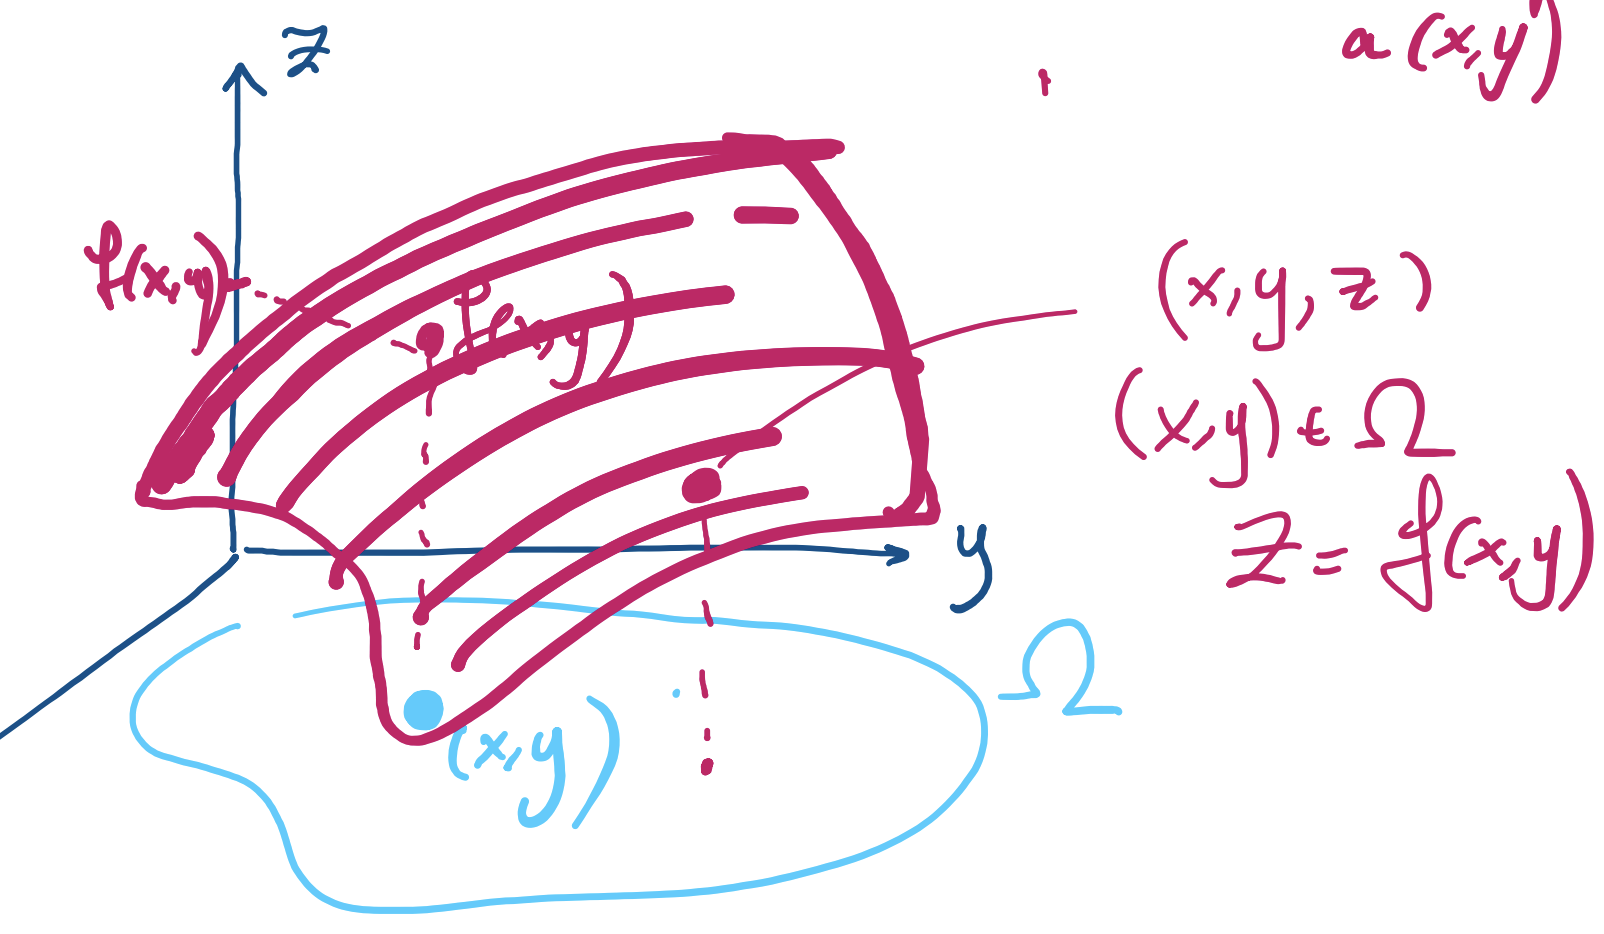
\includegraphics[width=5cm]{images/ess-funzioni-2-var.png}
\end{wrapfigure}
Ricordiamo che nell'analisi finora se $f: A \to \mathbb{R}$ con $A \subseteq \mathbb{R}$ chiamavamo il grafico di $f = \{(x,y) \in \mathbb{R}^2 \::\: x \in A, y = f(x)\}$ quindi abbiamo una linea nel piano $\mathbb{R}^2$.
Nell'analisi in 2 variabili abbiamo $f: \Omega \to \mathbb{R}$ con $\Omega \subseteq \mathbb{R}^2$ in questo caso per definire il grafico di $f = \{(x,y,z) \in \mathbb{R}^3 \::\: (x,y) \in \Omega, z = f(x,y)\}$. \\\\
Quindi il \textbf{grafico di f} è una superficie nello spazio dove $(x,y) \in \omega$ sa nel piano $xy$ mentre $z = f(x,y)$ è la quota (altezza) del punto della superficie che sta sopra a $(x,y)$.

\begin{observation}
Il dominio di $f: \mathbb{R}^n \to \mathbb{R}$ è uguale al il più grande sottoinsieme di $\mathbb{R}^n$ dove è definita (ha senso scriverla) la funzione.
\end{observation}

\hspace{-15pt}Possiamo anche prendere una funzione $f: \Omega \to \mathbb{R}$ con $\Omega \subseteq \mathbb{R}^n$ il grafico può essere generalizzato come $f= \{(x,y) \in \mathbb{R}^{n+1} \::\: x \in \Omega, y = f(x) \}$ dove $x \in \mathbb{R}^n$ è un vettore mentre $y \in \mathbb{R}$ è un numero.

\subsection{Insiemi di livello}
Per rappresentare meglio funzioni in n variabili si introduce il concetto di insiemi di livello (che nel caso di $n=2$ si dicono linee di livello). 
\begin{definition}
Sia $f: \mathbb{R}^2 \to \mathbb{R}$, e dato $\lambda \in \mathbb{R}$ (pensato come quota) \textbf{l'insieme di livello} corrispondente a $\lambda$ è il seguente insieme
$\{(x,y) \in \mathbb{R}^2 \::\: f(x,y) = \lambda\}$, è l'insieme quindi dei punti in $\mathbb{R}^2$ tale che la quota di f in questi punti è uguale a $\lambda$
\end{definition}
\hspace{-15pt}Possiamo vedere che $\{(x,y) \in \mathbb{R}^2 \::\: f(x,y) = \lambda\}$ (che viene chiamato anche insieme di livello $\lambda$ per $f$) è un sottoinsieme dello spazio di partenza tale che in questo sottoinsieme la funzione vale sempre $\lambda$.

\begin{example}\label{ess-insiemi-livello-1}
Prendiamo un $f(x,y) = x^2 + y^2$ con $f: \mathbb{R}^2 \to \mathbb{R}$, quindi con $(x,y) \to x^2 + y^2$ (quadrato della distanza di $(x,y)$ dall'origine). Gli insiemi di livello per questa funzione sono $\{(x,y) \in \mathbb{R}^2 \::\: x^2 + y^2 = \lambda\}$ per trovare questo insieme devo intersecare il grafico di $f$ con il pinao $z = \lambda$ e poi proietto sul piano $xy$.
\begin{itemize}
    \item Se $\lambda < 0 \to \O$.
    \item Se $\lambda = 0 \to (0,0)$.
    \item Se $\lambda > 0 \to$ trovo la circonferenza con centro in $(0,0)$ e raggio $\sqrt{\lambda}$.
\end{itemize}
Se scegliesti $\lambda = 1$ allora $\{(x,y) \in \mathbb{R}^2 \::\: x^2 + y^2 = 1\}$ avrei la circonferenza di raggio 1, mentre se scelgo $\lambda = 2$ allora $\{(x,y) \in \mathbb{R}^2 \:\: x^2+y^2 = 2\}$ avrei la circonferenza di raggio 2 in entrambi i casi con centro in $(0,0)$, questi sono quindi sottoinsiemi di $\mathbb{R}^2$. \\
L'insieme di livello $\lambda = \{$ punti di $\mathbb{R^2}$ tali che in questi punti la funzione vale $\lambda \}$.
\end{example}

\begin{example}\label{ess-insiemi-livello-2}
Prendiamo $f(x,y) = x\cdot y$. dato $\lambda \in \mathbb{R}$, l'insieme di livello $\lambda$ abbiamo che gli insiemi di livello sono $\{(x,y) \in \mathbb{R}^2 \::\: xy= \lambda\} \subseteq \mathbb{R}^2$, vediamo dunque di che insieme stiamo parlando:
\begin{itemize}
    \item Se $\lambda = 0 \::\: xy = 0$ questi punti sono quelli che stanno sugli assi ($x=0$ o $y=0$) allora $\{(x,y) \in \mathbb{R}^2 \::\: xy= \lambda\} = $asse y $\cup$ asse x.
    \item Se $\lambda > 0$ vuol dire che stiamo guardando $\{(x,y) \in \mathbb{R}^2 \::\: xy= \lambda\}$ con $y = \frac{\lambda}{x}$ e con $\lambda$ numero positivo, queste curve sono iperbole equilatere che sono nel 1° e nel 3° quadrante.
    \item Se $\lambda < 0$ abbiamo sempre $\{(x,y) \in \mathbb{R}^2 \::\: xy= \lambda\}$ ma questa volta con $y = \frac{\lambda}{x}$ con $\lambda < 0$ quindi saranno iperbole nel 2° e 3° quadrante.
\end{itemize}
\end{example}

\begin{example}\label{ess-insiemi-livello-3}
Prendiamo $f(x,y) = |x+y|$. Gli insiemi di livello di $\lambda$ con $\lambda \in \mathbb{R}$ in questo caso  saranno $\{(x,y) \in \mathbb{R}^2 \::\: f(x,y) = \lambda\} \subseteq \mathbb{R}^2 = \{(x,y) \in \mathbb{R}^2 \::\: |x+y| = \lambda\}$.
\begin{itemize}
    \item Se $\lambda < 0$ allora il valore assoluto non può essere mai uguale a $\lambda$ perché il valore assoluto e sempre positivo quindi $\to \O$.
    \item Se $\lambda = 0$ sto guardando $\{(x,y) \in \mathbb{R}^2 \::\: |x+y| = 0\}$ e questo è vero se $x+y = 0 \Longleftrightarrow y = -x$ quindi abbiamo la bisettrice del 2° e 4° quadrante.
    \item Se invece prendo $\lambda > 0$ sto cercando $\{(x,y) \in \mathbb{R}^2 \::\: |x+y| = \lambda\}$ ed in questo caso ci sono due possibilità, se $x+y > 0 \to y = \lambda - x$ mentre se $x+y < 0 \to -y = -\lambda-x$, quindi $\{(x,y) \in \mathbb{R}^2 \::\: |x+y| = \lambda\}$ con $\lambda > 0$ sarà $\{(x,y) \in \mathbb{R}^2 \::\: y = \lambda -x, y > -x \} \cup \{(x,y) \in \mathbb{R}^2 \::\: y = -x-\lambda, y < -x\}$.\\
    Dunque se per esempio $\lambda = 1 \to y = 1-x$ e $y = -1-x$ quindi ho l'unione di 2 rette.
\end{itemize}
\end{example}

\begin{figure}[h!]
\centering
\begin{subfigure}{.3\textwidth}
    \centering
    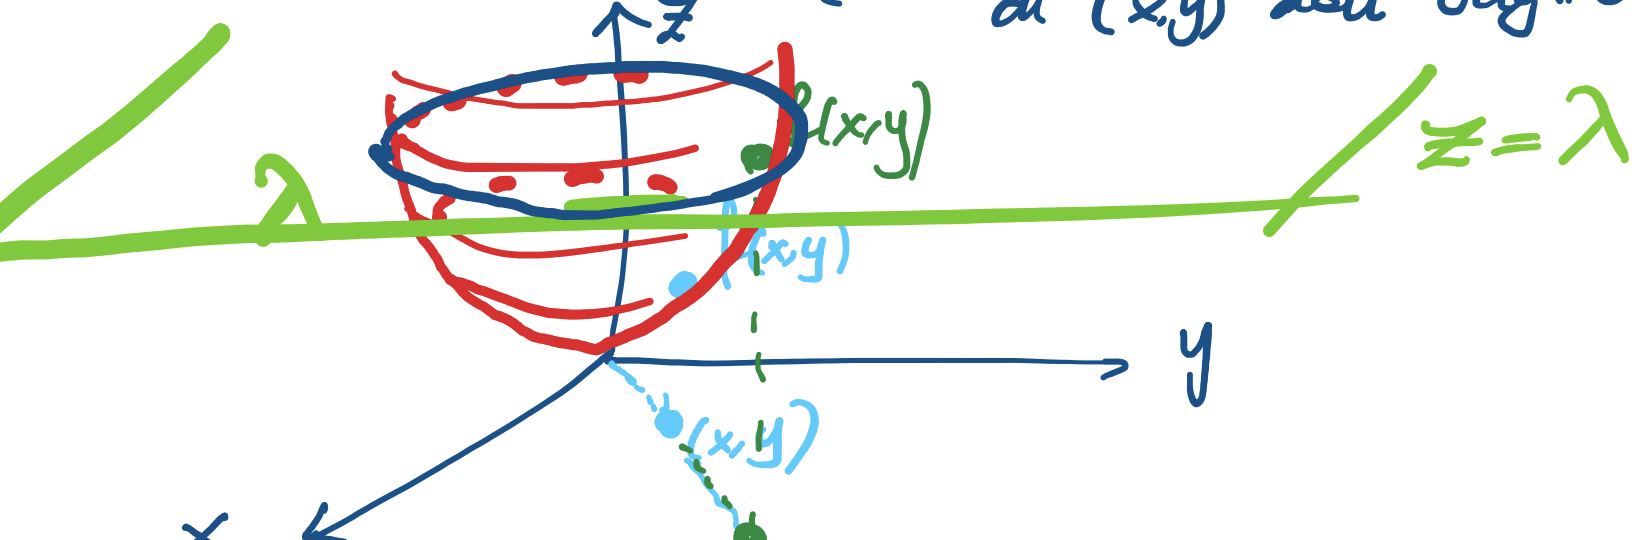
\includegraphics[width=5cm]{images/ess-insiemi-livello-1.png}
    \caption{Esempio \ref{ess-insiemi-livello-1}}
\end{subfigure}
\begin{subfigure}{.3\textwidth}
    \centering
    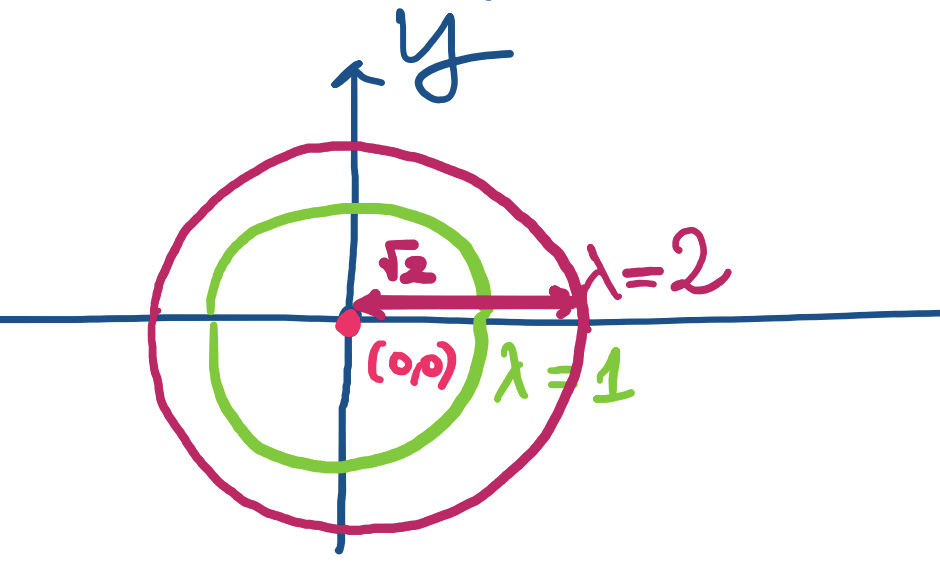
\includegraphics[width=3.7cm]{images/ess-insiemi-livello-2.png}
    \caption{Esempio \ref{ess-insiemi-livello-2}}
\end{subfigure}
\begin{subfigure}{.3\textwidth}
    \centering
    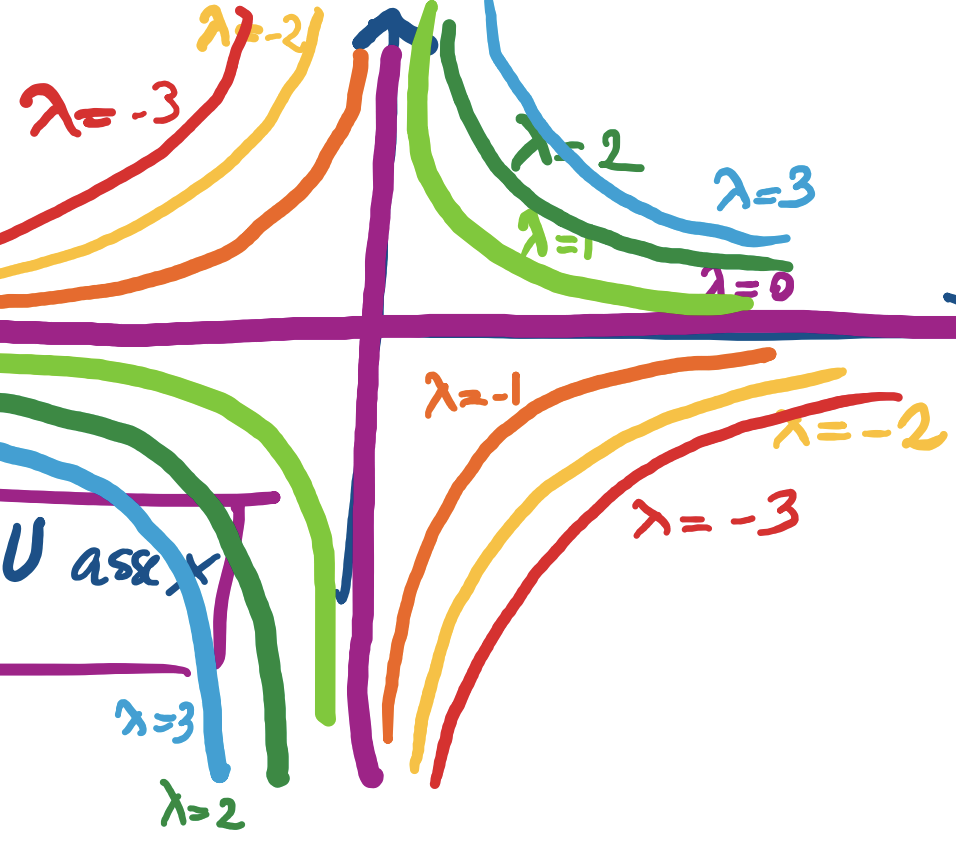
\includegraphics[width=3.3cm]{images/ess-insiemi-livello-3.png}
    \caption{Esempio \ref{ess-insiemi-livello-3}}
\end{subfigure}
\end{figure}